%% duodit_defense_fa.tex
%% Persian defense slides for DuoDiT thesis.
% !TEX TS-program = xelatex

\documentclass[aspectratio=169, 10pt]{beamer}
\usetheme[style=science]{lu}

\setlufootleft{دانشگاه تربیت مدرس}
\graphicspath{{graphics/}{../images/}{../images_samples/}{../img/}}

\usepackage{appendixnumberbeamer}
\usepackage{amsmath}
\usepackage{array}
\usepackage{animate}
\usepackage{multirow}
\usepackage{ragged2e}
\usepackage{xcolor}
\usetikzlibrary{arrows.meta,fit,shapes.geometric}

\title{بهبود مدل‌های انتشار مبتنی بر مبدل‌های بینایی برای تولید تصویر}
\author{مصطفی شهبازی دیل\\[0.4em]\small استاد راهنما: دکتر منصور رزقی آهق}
\institute{دانشکده علوم ریاضی}
\date{تابستان ۱۴۰۵}

% xepersian must be loaded late.
\usepackage{xepersian}

\settextfont[
    Path=../,
    Scale=1.08,
    BoldFont={XB NiloofarBd.ttf},
    ItalicFont={XB NiloofarIt.ttf},
    BoldItalicFont={XB NiloofarBdIt.ttf}
]{XB Niloofar.ttf}
\setpersiansansfont[
    Path=../,
    Scale=1.08,
    BoldFont={XB NiloofarBd.ttf},
    ItalicFont={XB NiloofarIt.ttf},
    BoldItalicFont={XB NiloofarBdIt.ttf}
]{XB Niloofar.ttf}
\setlatintextfont{Helvetica}

\newcommand{\duo}{\lr{DuoDiT}}
\newcommand{\dit}{\lr{DiT}}
\newcommand{\vit}{\lr{ViT}}
\newcommand{\fid}{\lr{FID}}
\newcommand{\kid}{\lr{KID}}
\newcommand{\lpips}{\lr{LPIPS}}
\newcommand{\cfg}{\lr{CFG}}
\newcommand{\imagenet}{\lr{ImageNet-1K}}
\newcommand{\metricdown}{\(\downarrow\)}
\newcommand{\compactitems}{\setlength{\itemsep}{0.35em}}
\newcommand{\smallcite}[1]{{\scriptsize\lr{[#1]}}}

\definecolor{DuoRed}{HTML}{C93B36}
\definecolor{DuoBlue}{HTML}{255C99}
\definecolor{DuoGreen}{HTML}{4C956C}
\definecolor{DuoGold}{HTML}{C49A32}
\definecolor{DuoInk}{HTML}{152238}
\definecolor{DuoSoft}{HTML}{F3F6FA}
\definecolor{DuoMist}{HTML}{EEF3F8}
\definecolor{DuoSidebar}{HTML}{10223D}
\definecolor{DuoSidebarMuted}{HTML}{9FB5D1}

\newlength{\DuoSidebarWidth}
\newlength{\DuoSidebarInnerWidth}
\newlength{\DuoSidebarLabelWidth}
\setlength{\DuoSidebarWidth}{0.145\paperwidth}
\setlength{\DuoSidebarInnerWidth}{0.116\paperwidth}
\setlength{\DuoSidebarLabelWidth}{0.102\paperwidth}
\setbeamersize{text margin left=.055\paperwidth, text margin right=.185\paperwidth}

\newif\ifDuoAppendix
\DuoAppendixfalse
\newcommand{\DuoDigit}[1]{%
    \ifcase\numexpr#1\relax
    ۰\or ۱\or ۲\or ۳\or ۴\or ۵\or ۶\or ۷\or ۸\or ۹\else \number\numexpr#1\relax\fi
}
\newcommand{\DuoCurrentChapterLabel}{%
    \ifDuoAppendix
        پیوست%
    \else
        \ifnum\value{section}=0
            نقشه ارائه%
        \else
            فصل \DuoDigit{\value{section}} از \DuoDigit{5}%
        \fi
    \fi
}
\newcommand{\DuoSidebarLine}[3]{%
    \begingroup
    \setlength{\fboxsep}{1.5pt}%
    \colorbox{#1}{%
        \parbox{\DuoSidebarLabelWidth}{%
            \begin{RTL}%
            \raggedleft{\color{#2}#3}%
            \end{RTL}%
        }%
    }\par
    \endgroup
}
\newcommand{\DuoSidebarRow}[2]{%
    \ifDuoAppendix
        \DuoSidebarLine{white}{DuoSidebar}{\tiny فصل \DuoDigit{#1}: #2}
    \else
        \ifnum\value{section}=#1
            \begingroup
            \setlength{\fboxsep}{2.2pt}%
            \colorbox{DuoGold}{%
                \parbox{\DuoSidebarLabelWidth}{%
                    \begin{RTL}%
                    \raggedleft{\color{DuoSidebar}\tiny\bfseries فصل \DuoDigit{#1}: #2}%
                    \end{RTL}%
                }%
            }\par
            \endgroup
        \else
            \DuoSidebarLine{white}{DuoSidebar}{\tiny فصل \DuoDigit{#1}: #2}
        \fi
    \fi
    \vspace{0.55ex}%
}
\newcommand{\DuoProgressRule}[1]{%
    \ifDuoAppendix
        {\color{DuoGold}\rule{0.018\paperwidth}{0.85mm}}%
    \else
        \ifnum\value{section}<#1
            {\color{DuoSidebarMuted!55}\rule{0.018\paperwidth}{0.85mm}}%
        \else
            {\color{DuoGold}\rule{0.018\paperwidth}{0.85mm}}%
        \fi
    \fi
}
\newcommand{\DuoSidebarPanel}{%
    \begingroup
    \setlength{\fboxsep}{0pt}%
    \colorbox{DuoSidebar}{%
        \parbox[t][\paperheight][t]{\DuoSidebarWidth}{%
            \centering
            \begin{minipage}[t][\paperheight]{\DuoSidebarInnerWidth}%
                \setRTL\raggedleft
                \vspace*{0.195\paperheight}%
                \DuoSidebarLine{white}{DuoSidebar}{\tiny\bfseries \DuoCurrentChapterLabel}
                \vspace{2.6ex}
                \DuoSidebarRow{1}{مقدمه و کلیات}
                \DuoSidebarRow{2}{کارهای مرتبط}
                \DuoSidebarRow{3}{روش پیشنهادی}
                \DuoSidebarRow{4}{نتایج و بحث}
                \DuoSidebarRow{5}{پیشنهادات و جمع‌بندی}
                \vfill
                \begin{flushleft}
                    \DuoProgressRule{5}\hspace{0.25em}%
                    \DuoProgressRule{4}\hspace{0.25em}%
                    \DuoProgressRule{3}\hspace{0.25em}%
                    \DuoProgressRule{2}\hspace{0.25em}%
                    \DuoProgressRule{1}%
                \end{flushleft}
                \vspace{1.0ex}
                \DuoSidebarLine{white}{DuoSidebar}{\tiny اسلاید \insertframenumber}
                \vspace*{0.040\paperheight}%
            \end{minipage}%
        }%
    }%
    \endgroup
}
\setbeamertemplate{blocks}[default]
\setbeamerfont{frametitle}{series=\bfseries,size=\Large}
\setbeamerfont{framesubtitle}{series=\mdseries,size=\normalsize}
\setbeamercolor{alerted text}{fg=DuoRed}
\setbeamercolor{background canvas}{bg=DuoMist}
\setbeamercolor{normal text}{fg=DuoInk,bg=white}
\setbeamercolor{frametitle}{fg=DuoInk,bg=white}
\setbeamercolor{framesubtitle}{fg=DuoBlue,bg=white}
\setbeamercolor{block title}{fg=white,bg=DuoBlue}
\setbeamercolor{block body}{fg=DuoInk,bg=white}
\setbeamercolor{duo sidebar}{fg=white,bg=DuoSidebar}
\setbeamercolor{duo sidebar active}{fg=DuoSidebar,bg=white}
\setbeamercolor{duo sidebar row}{fg=DuoSidebarMuted,bg=DuoSidebar}
\setbeamercolor{itemize item}{fg=DuoRed}
\setbeamercolor{itemize subitem}{fg=DuoGold}
\setbeamercolor{enumerate item}{fg=DuoRed}

\newcommand{\luRTLCenteredBlock}[2]{%
    \begin{minipage}[c]{#1}%
        \setRTL
        \centering
        #2%
    \end{minipage}%
}
\newcommand{\luRTLRightBlock}[2]{%
    \begin{minipage}[t]{#1}%
        \setRTL
        \raggedleft
        #2%
    \end{minipage}%
}
\newcommand{\duoTag}[2]{%
    \begingroup
    {\color{#1}\bfseries\scriptsize #2}%
    \endgroup
}
\newcommand{\duoMetric}[3]{%
    \begin{minipage}{0.29\linewidth}
        \centering
        {\Large\bfseries\lr{#1}}\\[-0.15em]
        {\scriptsize #2}\\[-0.1em]
        {\small\color{DuoGreen}\bfseries #3}
    \end{minipage}
}

% RTL frame title, title page, and closure patches derived from the local TMU template.
\makeatletter
\setbeamertemplate{background}{}
\setbeamertemplate{headline}{%
    \ifbeamer@plainframe\else
        \leavevmode
        \hbox to \paperwidth{\DuoSidebarPanel\hfill}%
        \vskip-\paperheight
    \fi
}
\setbeamertemplate{footline}{%
    \ifbeamer@plainframe\else
    \leavevmode
    \hbox to \paperwidth{%
        \hfill
        \begin{beamercolorbox}[
            wd=\dimexpr\paperwidth-\DuoSidebarWidth\relax,
            ht=2.6ex,
            dp=1.3ex
        ]{lu simple footline}%
            \hspace*{0.055\paperwidth}%
            \usebeamerfont{footline}%
            \beamer@lu@footleft
            \hfill
            \usebeamerfont{page number in head/foot}%
            \insertframenumber/\inserttotalframenumber
            \hspace*{0.035\paperwidth}%
        \end{beamercolorbox}%
    }%
    \vspace*{1.2ex}%
    \fi
}
\setbeamertemplate{frametitle}{%
    \nointerlineskip
    \hbox to \dimexpr\paperwidth-\DuoSidebarWidth\relax{%
        {\color{DuoGold}\rule{0.24\paperwidth}{0.7mm}}%
        {\color{DuoRed}\rule{0.13\paperwidth}{0.7mm}}%
        \hfill
    }%
    \vspace{2.25ex}%
    \begin{beamercolorbox}[wd=\paperwidth]{frametitle}%
        \hspace*{0.055\paperwidth}%
        \iflusidebar@active
        \iflusidebar@right\else \hspace*{\lusidebar@offset}\fi
        \fi
        \parbox[t]{\dimexpr\paperwidth-\DuoSidebarWidth-0.105\paperwidth\relax}{%
            \setRTL
            \raggedleft
            \usebeamerfont{frametitle}%
            \insertframetitle\strut\ %
            \usebeamerfont{framesubtitle}%
            \usebeamercolor[fg]{framesubtitle}%
            \insertframesubtitle%
        }\par%
    \end{beamercolorbox}%
}

\setbeamertemplate{title page}{%
    \begin{tikzpicture}[remember picture,overlay]
        \fill[darkblueLU] (current page.north west) rectangle (current page.south east);
        \node[anchor=south east,inner sep=0pt] at ($(current page.south east)+(-0.055\paperwidth,0.055\paperheight)$)
            {
\includegraphics[width=0.20\paperwidth]{components/tmu-logo}};
        \pgfmathsetlengthmacro{\R}{0.09\paperwidth}
        \node[anchor=east,text=white,font=\usebeamerfont{title}] at ($(current page.south east)+(-\R,0.64\paperheight)$)
            {\luRTLCenteredBlock{0.78\paperwidth}{\inserttitle}};
        \node[anchor=east,text=midblueLU,font=\usebeamerfont{author}] (authblock) at ($(current page.south east)+(-0.23\paperwidth,0.28\paperheight)$)
            {\luRTLRightBlock{0.58\paperwidth}{\AltSans\bfseries \insertauthor}};
        \node[anchor=north east,text=midblueLU,font=\usebeamerfont{institute}] at (authblock.south east)
            {\luRTLRightBlock{0.58\paperwidth}{\AltSans \insertinstitute\\\insertdate}};
    \end{tikzpicture}%
}

\renewcommand{\Closure}[3][]{%
    \pgfkeys{/closure, default, #1}
    \begin{tikzpicture}[remember picture,overlay]
    \fill[darkblueLU] (current page.north west) rectangle (current page.south east);
    \ifclosure@background
    \node[anchor=center,inner sep=0pt,opacity=0.22] at (current page.center)
        {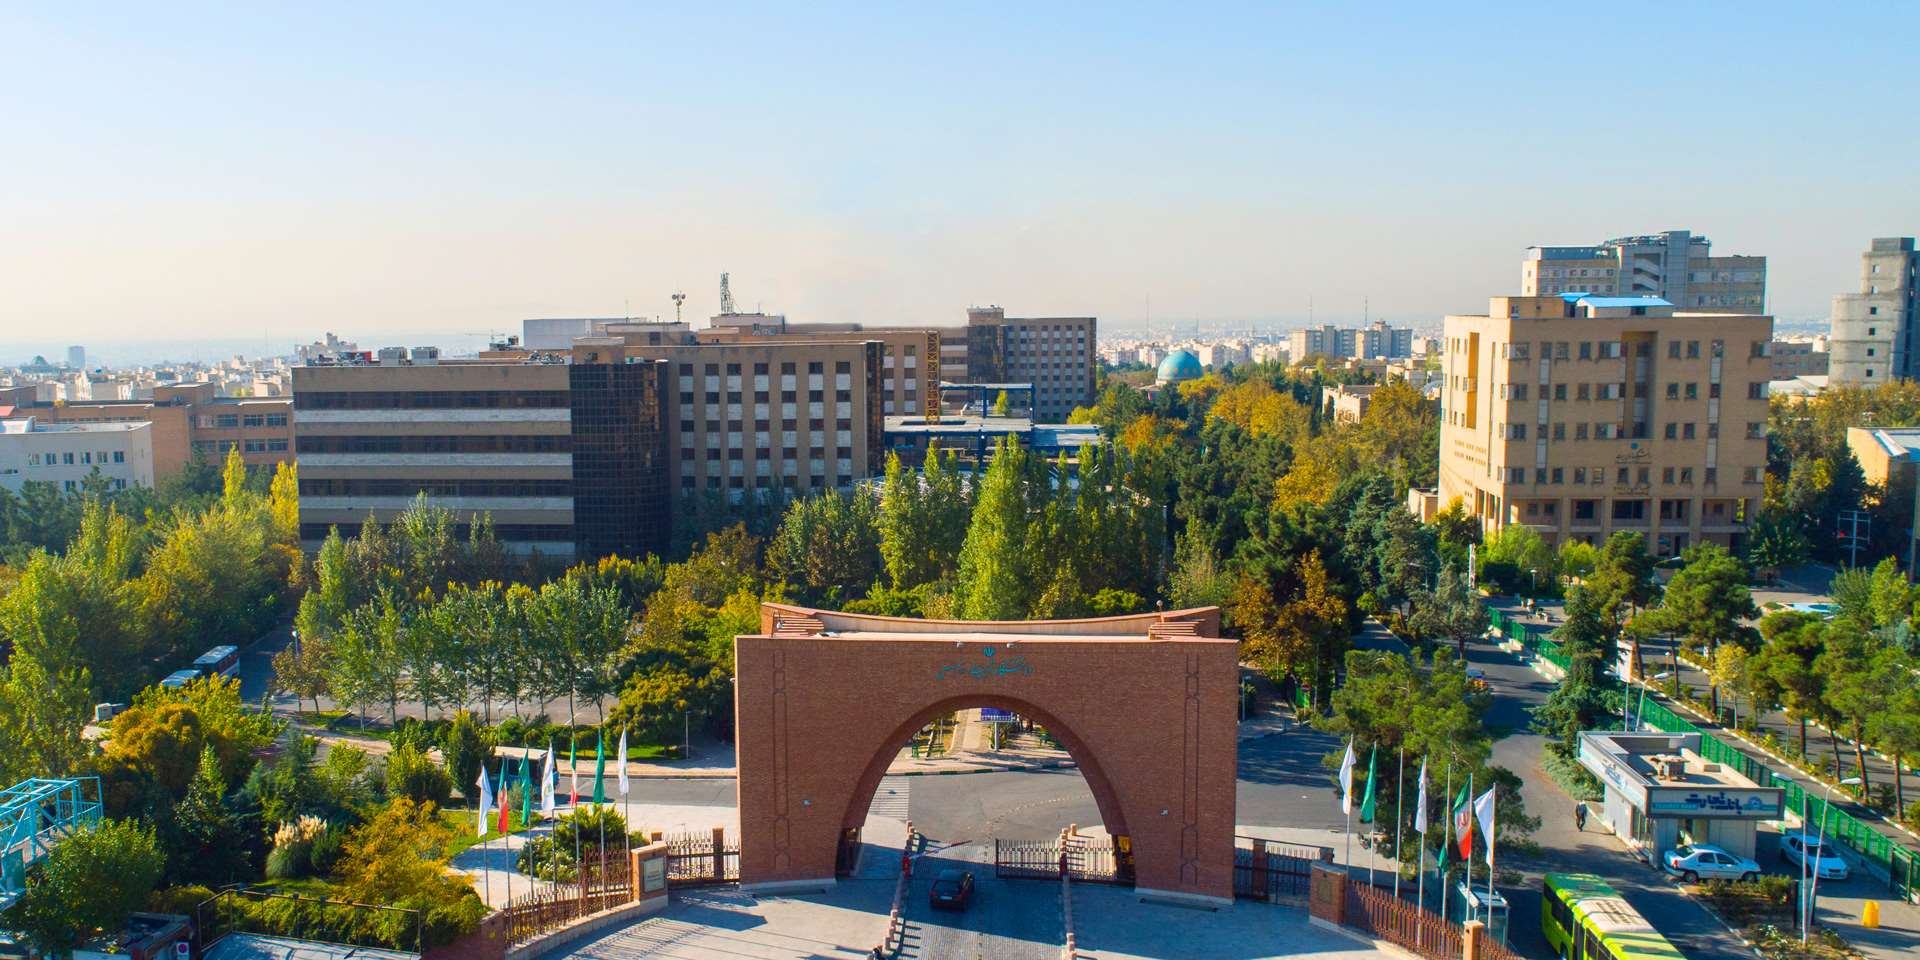
\includegraphics[width=\paperwidth,height=\paperheight]{components/tmu-1920-960}};
    \fi
    \ifclosure@circles
    \node[anchor=south east,inner sep=0pt,opacity=0.65] at (current page.south east)
        {
\includegraphics[height=\paperheight]{components/circles}};
    \fi
    \node[anchor=south east,inner sep=0pt] at ($(current page.south east)+(-0.04\paperwidth,0.045\paperheight)$)
        {
\includegraphics[width=0.18\paperwidth]{components/tmu-logo}};
    \node[anchor=east,text=white,font=\usebeamerfont{title}] at ($(current page.south east)+(-0.12\paperwidth,0.56\paperheight)$)
        {\luRTLCenteredBlock{0.70\paperwidth}{#2}};
    \node[anchor=east,text=midblueLU,font=\usebeamerfont{author}] at ($(current page.south east)+(-0.18\paperwidth,0.35\paperheight)$)
        {\luRTLRightBlock{0.60\paperwidth}{\AltSans #3}};
    \end{tikzpicture}%
}
\makeatother

\newenvironment{duobox}[1]{%
    \begin{block}{#1}\setlength{\parskip}{0.2em}\small
}{%
    \end{block}
}

\begin{document}

\begin{frame}[plain]
    \titlepage
\end{frame}

\begin{frame}{نقشه ارائه}
    \begin{columns}[T,onlytextwidth]
        % \begin{column}{0.38\textwidth}
        %     \centering
        %     \setlength{\fboxsep}{2pt}%
        %     \colorbox{white}{%
        %         \animategraphics[
        %             autoplay,
        %             loop,
        %             width=0.82\linewidth
        %         ]{12}{graphics/noise_to_image_frames/noise_to_image_}{0}{35}%
        %     }\par
        %     \vspace{0.25em}
        %     {\scriptsize\color{DuoBlue}\bfseries از نویز تا تصویر}\\[-0.1em]
        %     {\tiny\color{DuoInk!72} شهود مدل‌های انتشار برای شروع بحث}
        % \end{column}
        \begin{column}{0.58\textwidth}
            \begin{enumerate}
                \compactitems
                \item مقدمه و کلیات
                \item کارهای مرتبط
                \item روش پیشنهادی
                \item نتایج و بحث
                \item پیشنهادات و جمع‌بندی
            \end{enumerate}
        \end{column}
    \end{columns}
    \vspace{0em}
    % \begin{duobox}{}
    %     \footnotesize
    %     مدل انتشار از نویز آغاز می‌کند و گام‌به‌گام تصویر را می‌سازد؛ \duo{} این مسیر را با یک شاخه محلی سبک تقویت می‌کند.
    % \end{duobox}
\end{frame}

\section{مقدمه و کلیات}

\begin{frame}{یادگیری عمیق مولد تا مدل‌های انتشار}
    \begin{columns}[T,onlytextwidth]
        \begin{column}{0.48\textwidth}
            \centering
            \duoTag{DuoBlue}{خودرمزگذارها: فشرده‌سازی و بازسازی}\\[0.25em]
            \includegraphics[width=0.98\linewidth,height=0.28\textheight,keepaspectratio]{cae.png}
            \vspace{0.35em}
            \duoTag{DuoGold}{\lr{GAN}: رقابت مولد و متمایزگر}\\[0.2em]
            \includegraphics[width=0.98\linewidth,height=0.24\textheight,keepaspectratio]{gans.png}\\[-0.1em]
            {\scriptsize کیفیت بصری بالا، اما آموزش ناپایدار و خطر فروپاشی مود}\\[0.45em]
        \end{column}
        \begin{column}{0.48\textwidth}
            \begin{itemize}
                \compactitems
                \item خودرمزگذارها و سپس \lr{VAE}ها تصویر را در فضای نهان فشرده و بازسازی کردند. اما معمولاً جزئیات تیز و تنوع طبیعی تصویر را کامل حفظ نمی‌کنند.
                \item \lr{GAN}ها تولید تصویر را به رقابت دو شبکه تبدیل کردند و تصاویر شارپ‌تری ساختند.
                \item مدل‌های انتشار تولید را به فرایند تدریجی تبدیل کردند و کیفیت را پایدارتر کردند.
                \vspace{0.7em}
                \duoTag{DuoGreen}{\lr{Diffusion}: حذف نویز تدریجی}\\[0.2em]
                
\includegraphics[width=0.15\linewidth]{noise_to_image_frames/noise_to_image_0.png}\hspace{0.25em}
                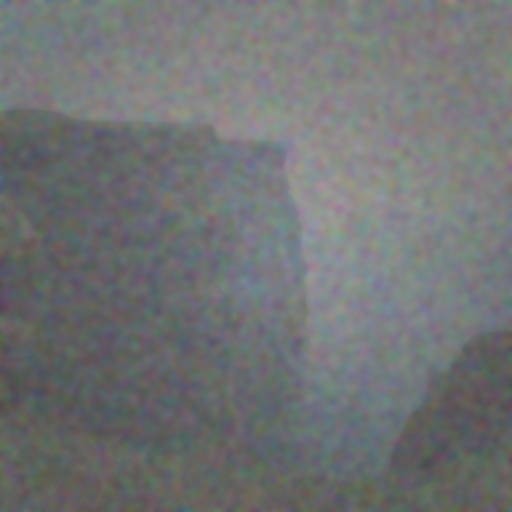
\includegraphics[width=0.15\linewidth]{noise_to_image_frames/noise_to_image_12.png}\hspace{0.25em}
                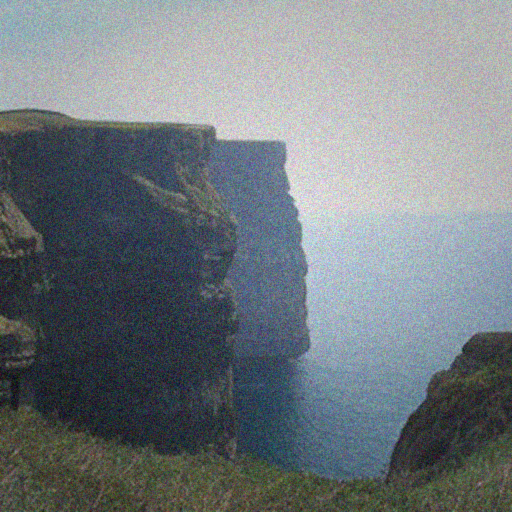
\includegraphics[width=0.15\linewidth]{noise_to_image_frames/noise_to_image_24.png}\hspace{0.25em}
                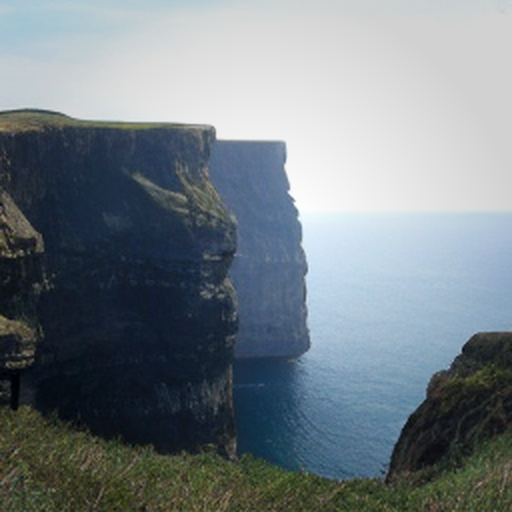
\includegraphics[width=0.15\linewidth]{noise_to_image_frames/noise_to_image_35.png}\\[-0.1em]
                \vspace{0.7em}
                {\scriptsize کیفیت و پایداری بهتر، اما نمونه‌برداری و آموزش پرهزینه}
            \end{itemize}
        \end{column}
    \end{columns}
\end{frame}

\begin{frame}{مجموعه‌داده \imagenet{}}
    \begin{columns}[T,onlytextwidth]
        \begin{column}{0.48\textwidth}
            \begin{itemize}
                \compactitems
                \item \imagenet{} یک معیار مرجع گسترده برای تولید تصویر شرطی است.
                \item شامل هزار کلاس شیء با تنوع زیاد در ظاهر، زمینه و زاویه دید است.
                \item در این پژوهش، تولید کلاس‌محور در وضوح \lr{256x256} بررسی می‌شود.
                \item دشواری اصلی: مدل باید هم ساختار معنایی کلاس و هم جزئیات بصری را حفظ کند.
            \end{itemize}
        \end{column}
        \begin{column}{0.48\textwidth}
            \centering
            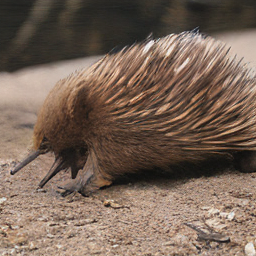
\includegraphics[width=0.30\linewidth]{028102-class0102.png}
            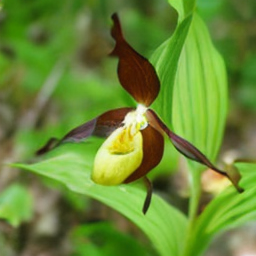
\includegraphics[width=0.30\linewidth]{009986-class0986.png}
            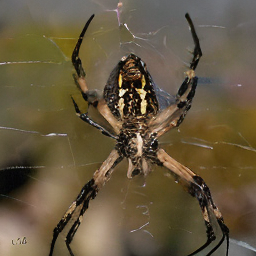
\includegraphics[width=0.30\linewidth]{028072-class0072.png}\\[-0.1em]
            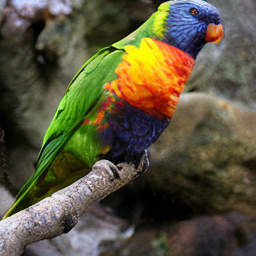
\includegraphics[width=0.30\linewidth]{023090-class0090.png}
            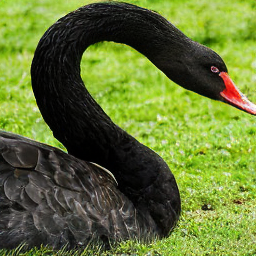
\includegraphics[width=0.30\linewidth]{044100-class0100.png}
            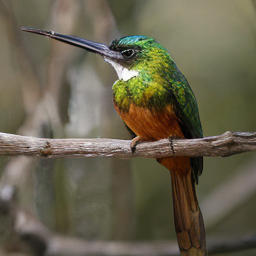
\includegraphics[width=0.30\linewidth]{037095-class0095.png}
            \vspace{0.35em}
        \end{column}
    \end{columns}
\end{frame}

\begin{frame}{ارزیابی مدل‌های تولید تصویر}
    \begin{columns}[T,onlytextwidth]
        \begin{column}{0.32\textwidth}
            \begin{duobox}{\fid{}}
                فاصله توزیعی بین ویژگی‌های تصاویر واقعی و تولیدی؛ برای سنجش شباهت کلی توزیع.
            \end{duobox}
        \end{column}
        \begin{column}{0.32\textwidth}
            \begin{duobox}{\kid{}}
                معیار توزیعی مبتنی بر هسته؛ برای مقایسه پایدارتر مجموعه‌های واقعی و تولیدی.
            \end{duobox}
        \end{column}
        \begin{column}{0.32\textwidth}
            \begin{duobox}{\lpips{}}
                فاصله ادراکی بین تصویرها در فضای ویژگی شبکه عمیق؛ مکمل معیارهای توزیعی.
            \end{duobox}
        \end{column}
    \end{columns}
    \vspace{0.65em}
    \begin{itemize}
        \compactitems
        \item مقدار کمتر در هر سه معیار بهتر است.
        \item \fid{} و \kid{} رفتار کل مجموعه نمونه‌ها را می‌سنجند؛ \lpips{} به شباهت ادراکی نزدیک‌تر است.
        \item تفسیر نهایی باید همراه با نمونه‌های تصویری و مطالعه انسانی انجام شود.
    \end{itemize}
\end{frame}

\section{کارهای مرتبط}

\begin{frame}{تاریخچه کارهای مرتبط}
    \centering
    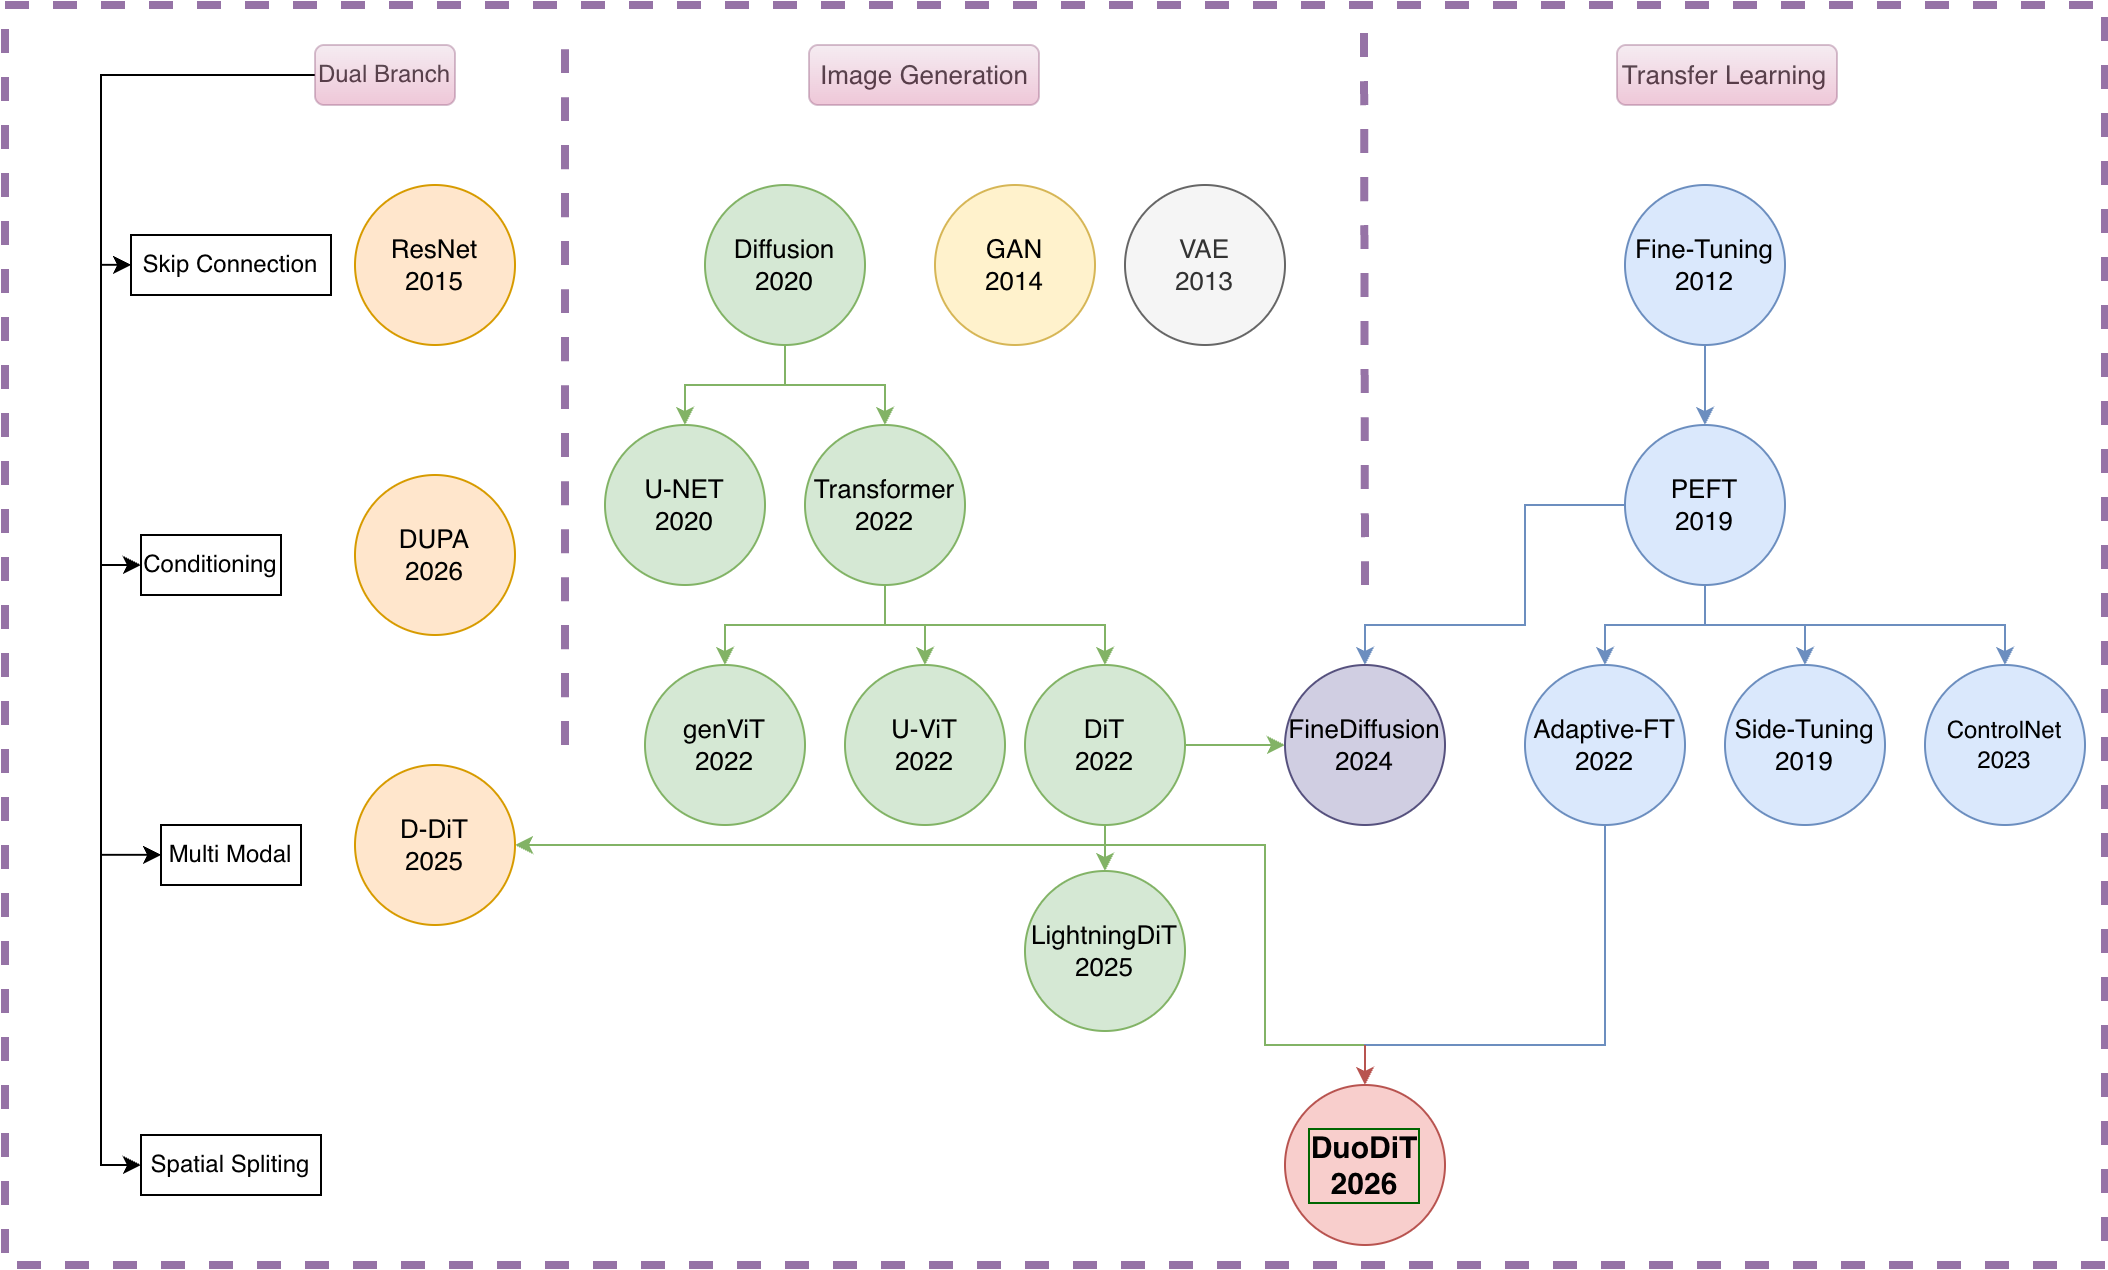
\includegraphics[width=0.96\linewidth,height=0.78\textheight,keepaspectratio]{new-his-to-duodit.drawio.png}
    \vspace{0.2em}
\end{frame}

\begin{frame}{فرمول‌بندی انتشار}
    \begin{columns}[onlytextwidth]
        \begin{column}{0.52\textwidth}
            \begin{itemize}
                \compactitems
                \item در \lr{DDPM} داده با یک زنجیره مارکوف به نویز تبدیل می‌شود.
                \item مسیر معکوس با شبکه‌ای یاد گرفته می‌شود که نویز را پیش‌بینی می‌کند.
                \item شرط کلاس یا متن در تابع \(\epsilon_\theta(x_t,t,c)\) وارد می‌شود.
            \end{itemize}
        \end{column}
        \begin{column}{0.44\textwidth}
            \[
            q(x_t|x_{t-1})=\mathcal{N}(\sqrt{\alpha_t}x_{t-1},(1-\alpha_t)I)
            \]
            \[
            p_\theta(x_{t-1}|x_t)=\mathcal{N}(\mu_\theta,\Sigma_\theta)
            \]
        \end{column}
    \end{columns}
    \vspace{0.4em}
    \begin{duobox}{توضیح}
        تابع نویزی کردن عکس ثابت می‌ماند؛ نقطه رقابت، طراحی شبکه حذف نویز و نحوه شرط‌گذاری است.
    \end{duobox}
\end{frame}

\begin{frame}{\vit{}: تصویر به‌عنوان توالی توکن}
    \begin{columns}[onlytextwidth]
        \begin{column}{0.45\textwidth}
            \centering
            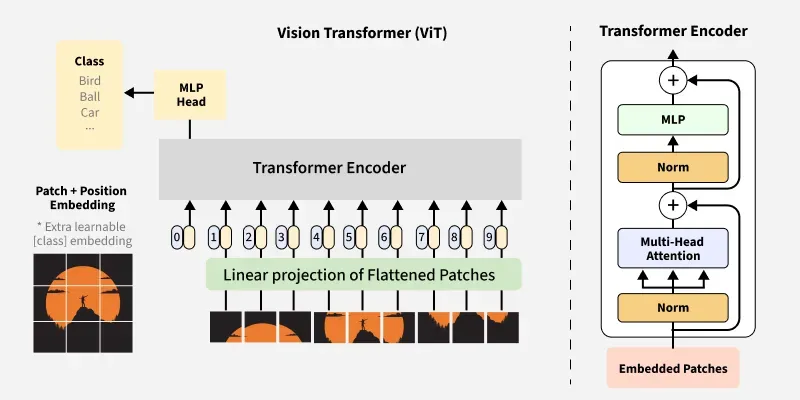
\includegraphics[width=0.95\linewidth]{vit.png}
        \end{column}
        \begin{column}{0.51\textwidth}
            \[
                N=\frac{HW}{P^2},\quad
                z_0^i=E x_p^i + E_{pos}^i
            \]
            \[
                \text{Attention}(Q,K,V)=
                \text{softmax}\left(\frac{QK^T}{\sqrt{d_k}}\right)V
            \]
            \begin{itemize}
                \compactitems
                \item پچ‌ها نقش توکن‌های ورودی را دارند.
                \item توجه، رابطه‌های دوربرد بین نواحی تصویر را مدل می‌کند.
            \end{itemize}
        \end{column}
    \end{columns}
\end{frame}

\begin{frame}{\dit{}: مبدل به‌عنوان حذف‌کننده نویز}
    \begin{columns}[onlytextwidth]
        \begin{column}{0.49\textwidth}
            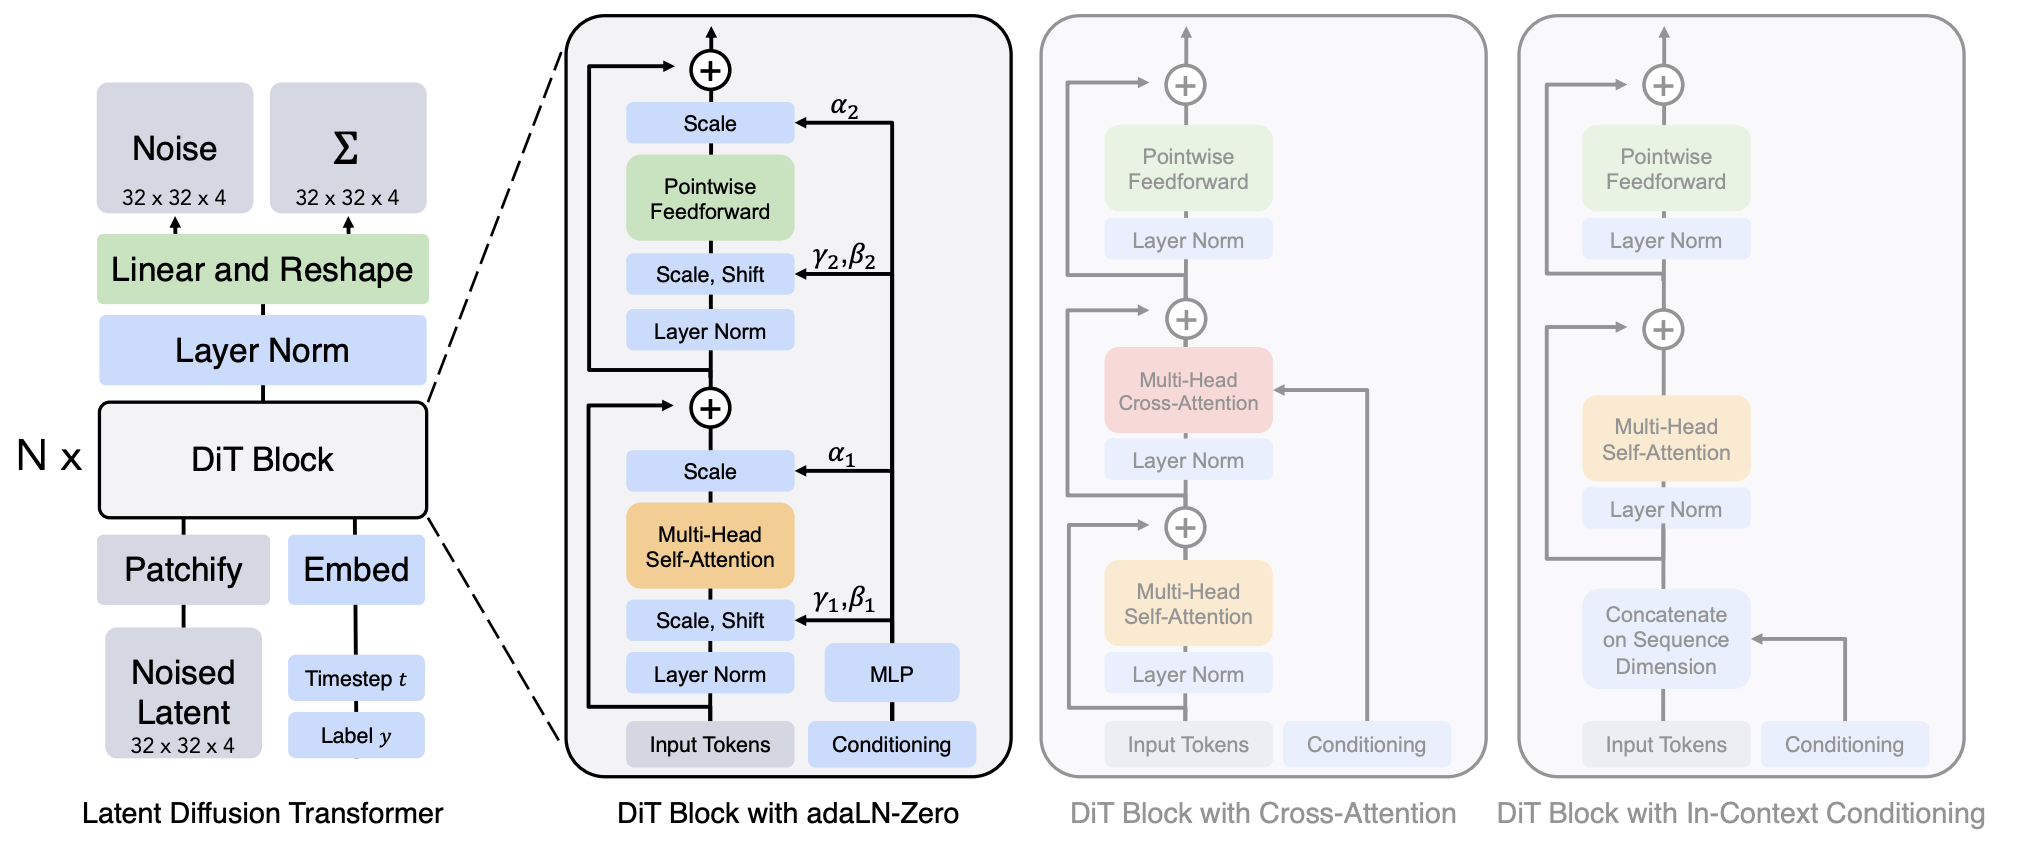
\includegraphics[width=\linewidth]{base_dit.png}
        \end{column}
        \begin{column}{0.47\textwidth}
            \begin{itemize}
                \compactitems
                \item ورودی در فضای نهان \lr{VAE} پردازش می‌شود.
                \item پچ‌های نهان وارد بلوک‌های مبدل می‌شوند.
                \item زمان و کلاس با \lr{adaLN-Zero} به بلوک‌ها تزریق می‌شوند.
            \end{itemize}
            \vspace{0.3em}
            \[
                \text{\lr{adaLN}}(h,t,c)=
                \gamma(t,c)\odot \text{\lr{Norm}}(h)+\beta(t,c)
            \]
        \end{column}
    \end{columns}
\end{frame}

\begin{frame}{معماری‌های دوشاخه‌ای: اتصال باقی‌مانده}
    \begin{columns}[T,onlytextwidth]
        \begin{column}{0.48\textwidth}
            \centering
            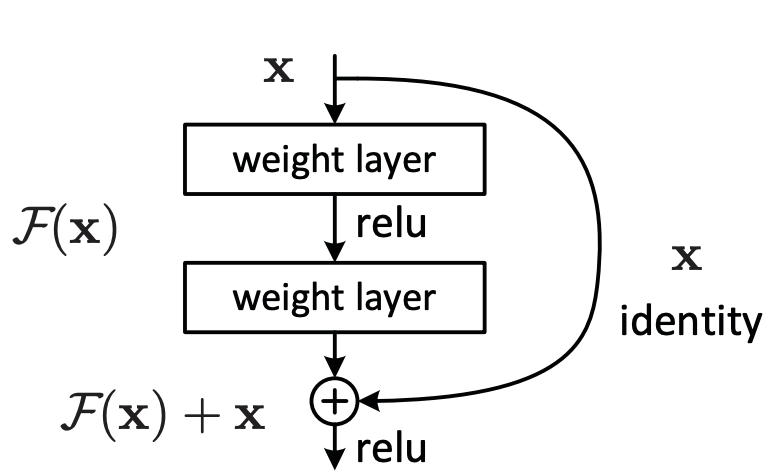
\includegraphics[width=0.94\linewidth,height=0.54\textheight,keepaspectratio]{resnet-skipconnection.png}
            \vspace{0.2em}
            {\scriptsize \lr{Deep Residual Learning for Image Recognition}}
        \end{column}
        \begin{column}{0.48\textwidth}
            \begin{itemize}
                \compactitems
                \item مسیر هویتی، اطلاعات اولیه را بدون تخریب حفظ می‌کند.
                \item مسیر باقی‌مانده، اصلاح یا تکمیل ویژگی‌ها را یاد می‌گیرد.
                \item این ایده مبنای بسیاری از ادغام‌های شاخه‌ای و جمع باقی‌مانده است.
            \end{itemize}
        \end{column}
    \end{columns}
\end{frame}

\begin{frame}{معماری‌های دوشاخه‌ای: توجه محلی و سراسری}
    \centering
    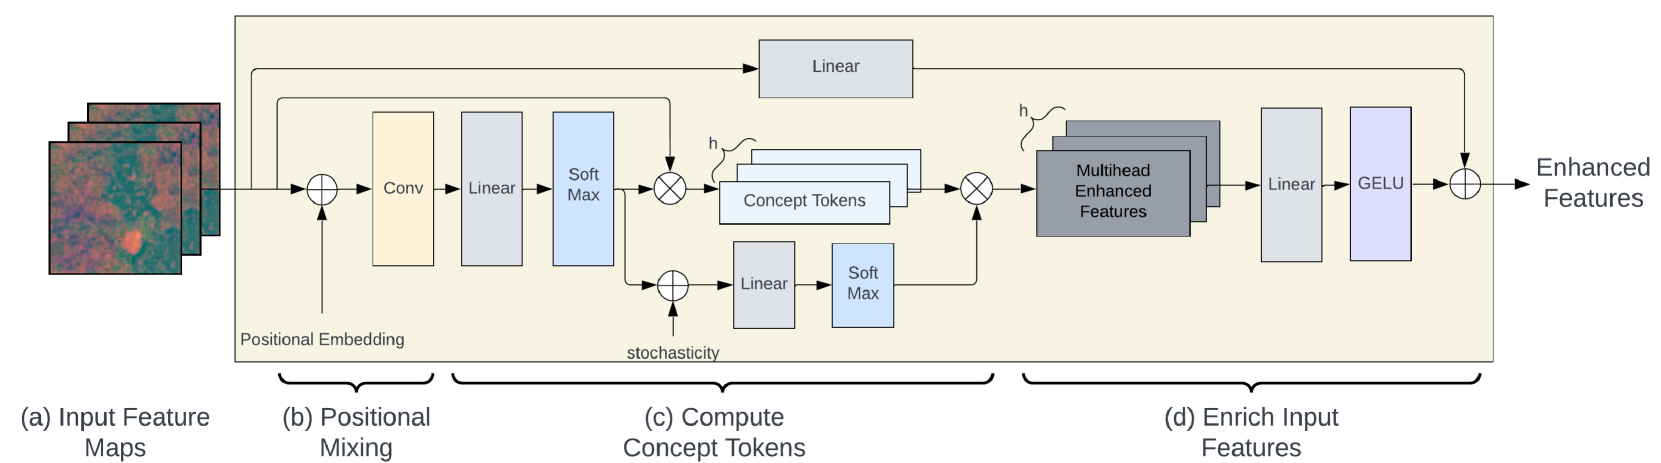
\includegraphics[width=0.96\linewidth,height=0.45\textheight,keepaspectratio]{unfied-local-global.png}
    \vspace{0.25em}

    \begin{columns}[T,onlytextwidth]
        \begin{column}{0.48\textwidth}
            \begin{duobox}{مسیر محلی}
                استخراج نشانه‌های مکانی، مفهوم‌های موضعی و ویژگی‌های ریزدانه از نقشه ویژگی.
            \end{duobox}
        \end{column}
        \begin{column}{0.48\textwidth}
            \begin{duobox}{مسیر سراسری}
                تعامل توجه چندسری برای غنی‌سازی ویژگی‌ها و ترکیب زمینه کلی تصویر.
            \end{duobox}
        \end{column}
    \end{columns}
    \vspace{0.25em}
    {\scriptsize \lr{Unified Local and Global Attention Interaction Modeling for Vision Transformers}}
\end{frame}

\begin{frame}{معماری‌های دوشاخه‌ای در انتشار: \lr{D-DiT} و \lr{DUPA}}
    \begin{columns}[T,onlytextwidth]
        \begin{column}{0.49\textwidth}
            \centering
            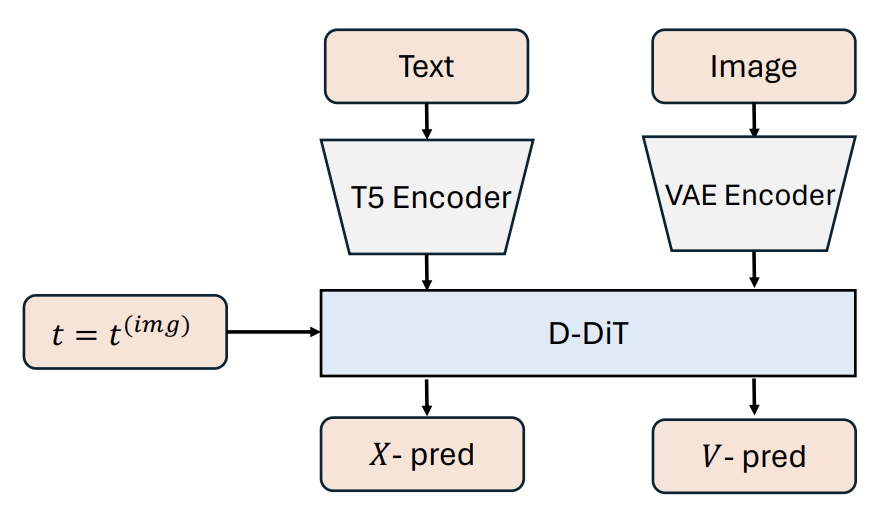
\includegraphics[width=0.98\linewidth,height=0.58\textheight,keepaspectratio]{d-dit.png}
            \vspace{0.2em}
            {\scriptsize \lr{Dual Diffusion for Unified Image Generation and Understanding}}
        \end{column}
        \begin{column}{0.49\textwidth}
            \centering
            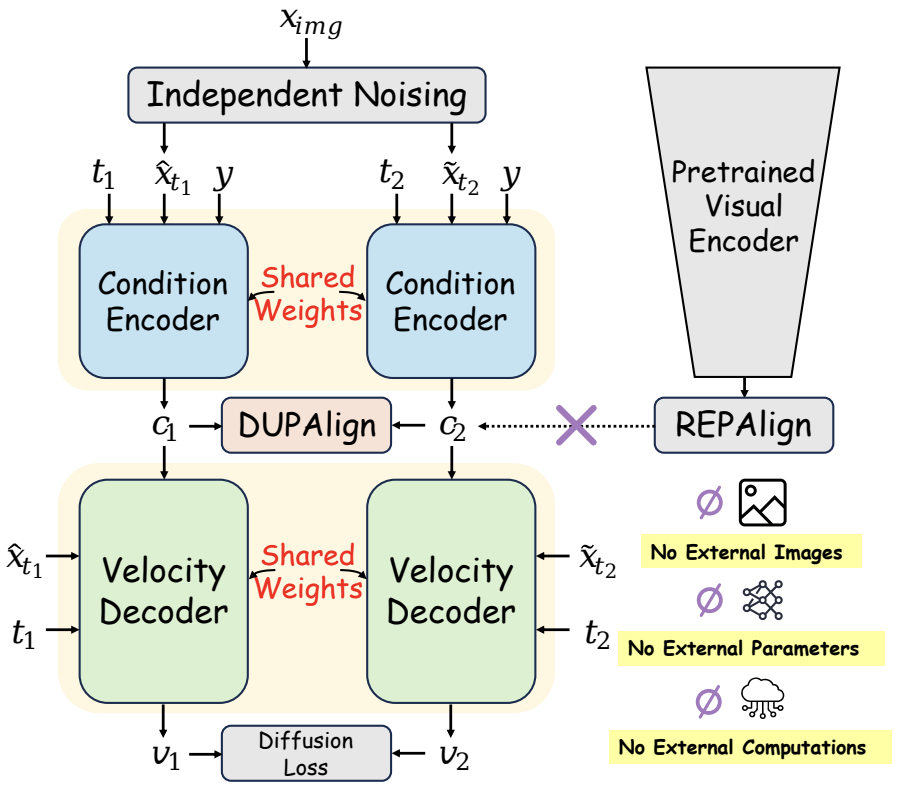
\includegraphics[width=0.95\linewidth,height=0.64\textheight,keepaspectratio]{dupa-arch.png}
            \vspace{0.15em}
            {\scriptsize \lr{DUAL-PATH CONDITION ALIGNMENT FOR DIFFUSION TRANSFORMERS}}
        \end{column}
    \end{columns}
\end{frame}

\begin{frame}{\lr{LightningDiT} و \lr{FineDiffusion}}
    \begin{columns}[onlytextwidth]
        \begin{column}{0.49\textwidth}
            \begin{duobox}{\lr{LightningDiT}}
                مسیر قدرتمند برای بهبود آموزش و بازسازی نمایش نهان؛ در این پایان‌نامه، مبنای قوی از نظر \fid{} است.
            \end{duobox}
            \begin{duobox}{\lr{FineDiffusion}}
                تنظیم پارامتر-کارا با تمرکز بر سازگار کردن مولفه‌های محدود در مدل انتشار شرطی.
            \end{duobox}
        \end{column}
        \begin{column}{0.47\textwidth}
            \begin{itemize}
                \compactitems
                \item این کارها نشان می‌دهند کیفیت، فقط تابع تعداد پارامتر نیست.
                \item برای \dit{} منجمد، مسیر مکمل می‌تواند تزریق ویژگی‌های محلی باشد.
                \item پرسش این پژوهش: آیا شاخه دوم سبک می‌تواند کیفیت ادراکی را بهتر کند؟
            \end{itemize}
        \end{column}
    \end{columns}
\end{frame}

\begin{frame}{شکاف پژوهشی}
    \begin{columns}[onlytextwidth]
        \begin{column}{0.31\textwidth}
            \begin{duobox}{مبدل‌های انتشار}
                قوی و مقیاس‌پذیر، اما تنظیم کامل آن‌ها پرهزینه است.
            \end{duobox}
        \end{column}
        \begin{column}{0.31\textwidth}
            \begin{duobox}{روش‌های \lr{PEFT}}
                سبک‌تر، اما همیشه برای جزئیات مکانی کافی نیستند.
            \end{duobox}
        \end{column}
        \begin{column}{0.31\textwidth}
            \begin{duobox}{مسیرهای چندمقیاسی}
                برای محلیت مفیدند، اما باید با طول توکنی \dit{} سازگار شوند.
            \end{duobox}
        \end{column}
    \end{columns}
    % \vspace{0.75em}
    % \centering
    % \duoTag{DuoRed}{پاسخ پیشنهادی} \hspace{0.5em}
    % \duo{} = بدنه منجمد \dit{} + شاخه وضوح‌بالا + توکن کلاس محلی + ادغام نهایی
\end{frame}

\section{روش پیشنهادی}

\begin{frame}{نمای کلی}
    \centering
    \includegraphics[width=0.98\linewidth]%,height=0.78\textheight,keepaspectratio,trim=0 210 0 230,clip]
    {duodit-components-benefits.drawio.png}
    \vspace{0.3em}

    {\small نمای کلی مدل پیشنهادی و دستاوردها}
\end{frame}

\begin{frame}{معماری \duo{}}
    \centering
    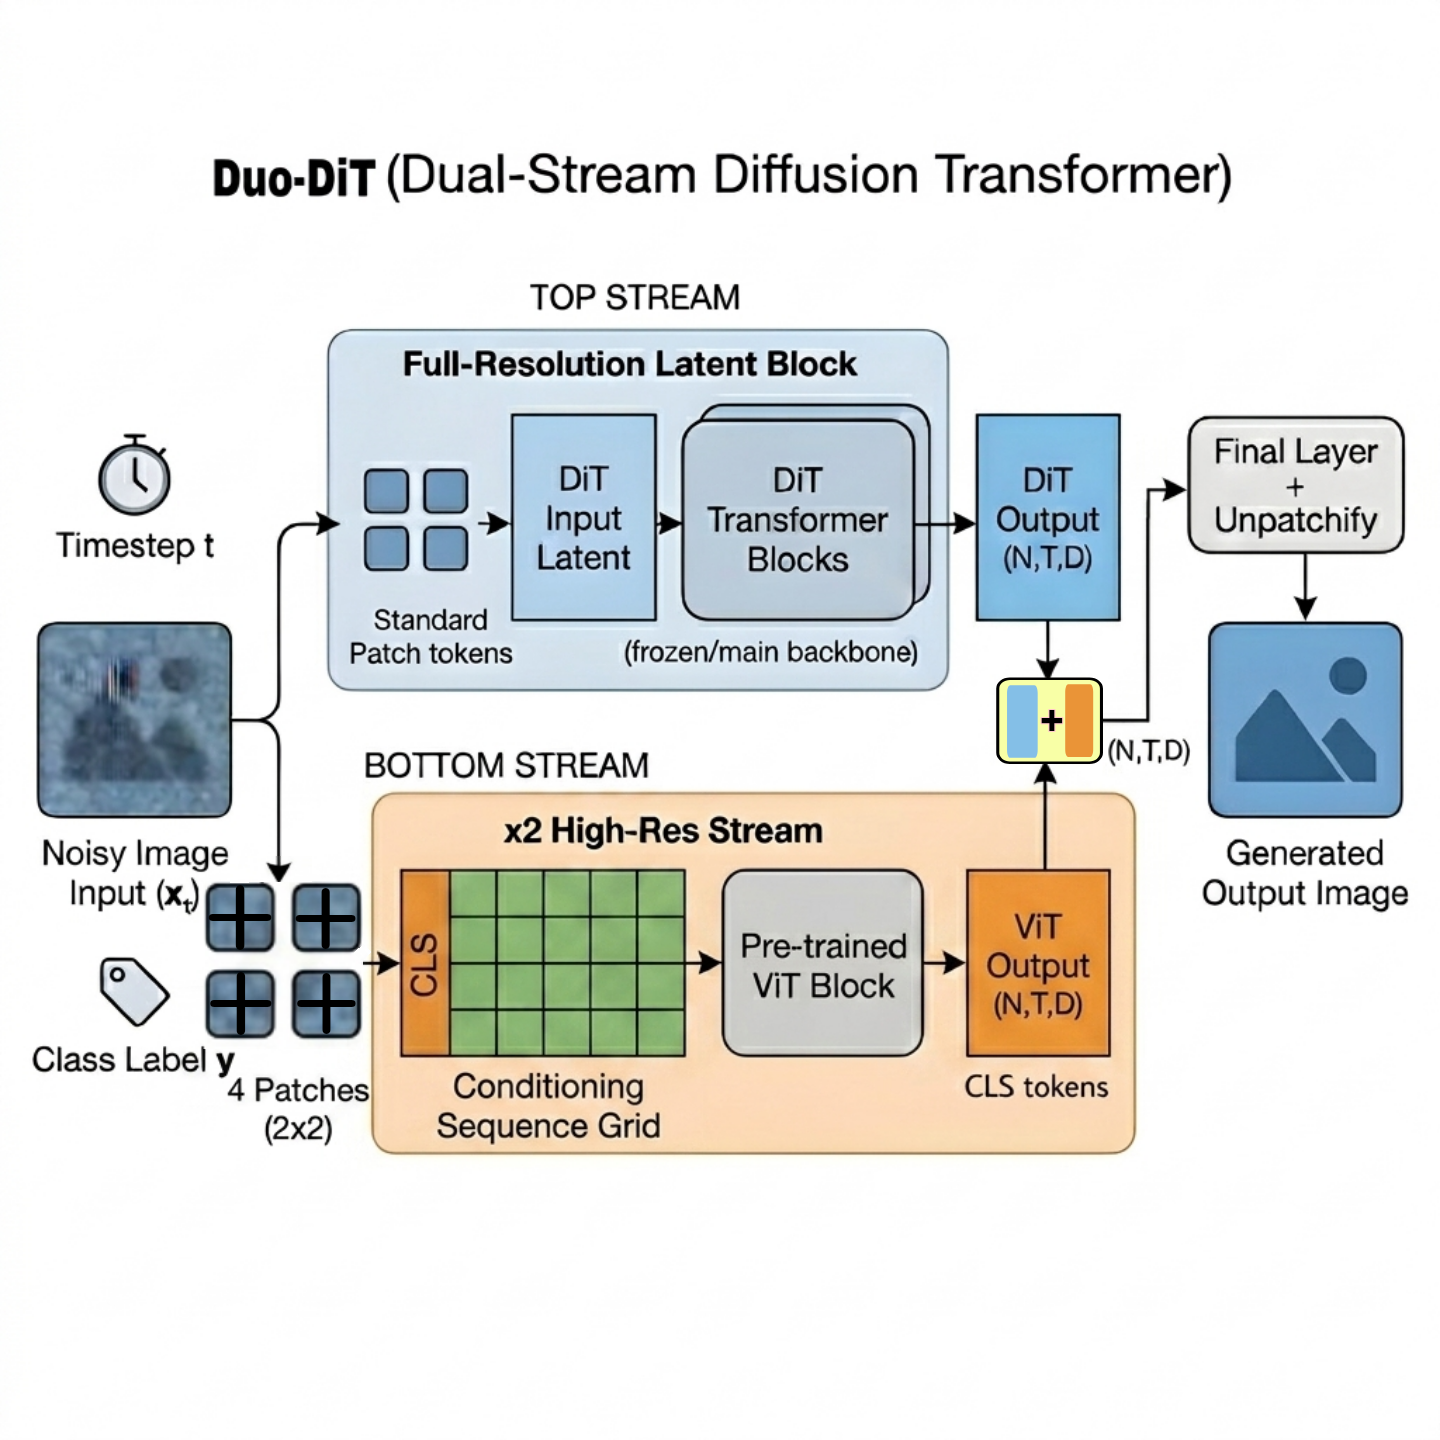
\includegraphics[width=0.98\linewidth,height=0.78\textheight,keepaspectratio,trim=0 210 0 230,clip]{proposed_architecture_overview.png}
    \vspace{0.3em}

    {\small بدنه اصلی دانش سراسری را حفظ می‌کند؛ شاخه \lr{x2} ویژگی‌های ریزدانه را استخراج و هم‌تراز می‌کند.}
\end{frame}

\begin{frame}{بدنه منجمد \lr{DiT-XL/2}}
    \begin{columns}[onlytextwidth]
        \begin{column}{0.50\textwidth}
            \begin{itemize}
                \compactitems
                \item وزن‌های بدنه اصلی منجمد می‌مانند.
                \item دانش پیش‌آموزش‌دیده و ساختار معنایی تصویر حفظ می‌شود.
                \item هزینه گرادیان و ذخیره‌سازی کاهش می‌یابد.
            \end{itemize}
        \end{column}
        \begin{column}{0.46\textwidth}
            \begin{duobox}{مشخصات پایه}
                \begin{latin}
                \begin{tabular}{lc}
                    \toprule
                    Backbone & DiT-XL/2\\
                    Depth & 28\\
                    Hidden dim & 1152\\
                    Heads & 16\\
                    Main patch & 2\\
                    \bottomrule
                \end{tabular}
                \end{latin}
            \end{duobox}
        \end{column}
    \end{columns}
    \[
        H_{\text{backbone}}^{(L)}=\mathcal{F}_{\theta}(x_t,t,y),\quad \theta \ \text{ثابت}
    \]
\end{frame}

\begin{frame}{شاخه \lr{x2}: افزایش وضوح توکنی}
    \begin{columns}[onlytextwidth]
        \begin{column}{0.52\textwidth}
            \begin{itemize}
                \compactitems
                \item شاخه اصلی با پچ \(2\times2\) کار می‌کند.
                \item شاخه دوم با پچ \(1\times1\) چهار برابر توکن تولید می‌کند.
                \item مسئله: خروجی شاخه دوم باید از \(4T\) توکن به \(T\) توکن برسد.
            \end{itemize}
        \end{column}
        \begin{column}{0.44\textwidth}
            \centering
            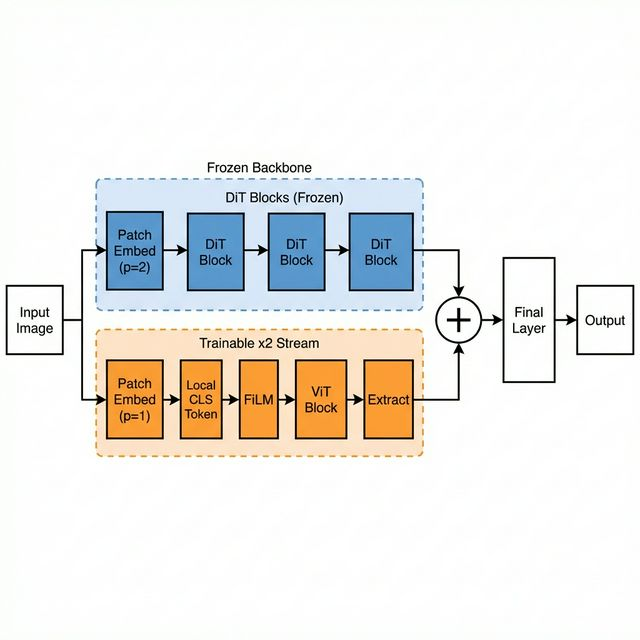
\includegraphics[width=0.96\linewidth]{proposed_x2_dit_architecture_overview.png}
        \end{column}
    \end{columns}
    \[
        Z_{x2}=\mathcal{E}_{x2}(x_t),\quad Z_{x2}\in\mathbb{R}^{N\times4T\times D}
    \]
\end{frame}

\begin{frame}{\vit{} به‌عنوان خبره شاخه دوم}
    \begin{columns}[onlytextwidth]
        \begin{column}{0.51\textwidth}
            \begin{itemize}
                \compactitems
                \item بلوک شاخه دوم از \lr{vit\_large\_patch16\_224} مقداردهی اولیه می‌شود.
                \item پروجکشن‌های خطی، بعد \vit{} را با بعد \dit{} سازگار می‌کنند.
                \item هدف: استفاده از بازنمایی‌های بصری آماده برای جزئیات محلی.
            \end{itemize}
        \end{column}
        \begin{column}{0.45\textwidth}
            \[
                U=\mathcal{T}_{\phi}(\text{Flatten}([\text{Group}(Z_{x2});C]))
            \]
            \[
                H_{x2}=\text{SelectClassToken}(U)
            \]
            \[
                H_{x2}\in\mathbb{R}^{N\times T\times D}
            \]
        \end{column}
    \end{columns}
\end{frame}

\begin{frame}{توکن کلاس محلی}
    \begin{columns}[onlytextwidth]
        \begin{column}{0.48\textwidth}
            \centering
            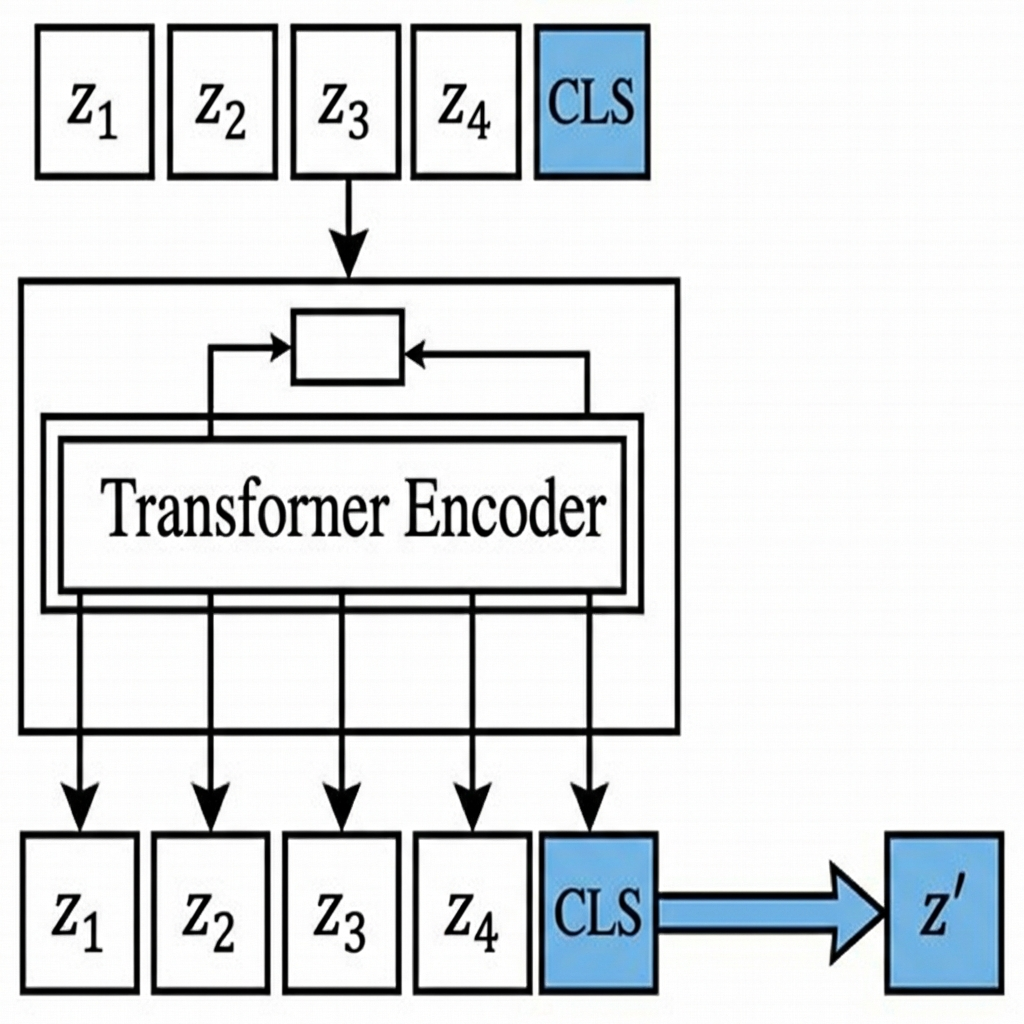
\includegraphics[width=0.95\linewidth]{local_cls_mechanism.png}
        \end{column}
        \begin{column}{0.48\textwidth}
            \begin{itemize}
                \compactitems
                \item هر چهار توکن محلی با یک توکن یادگیرنده پردازش می‌شوند.
                \item خروجی توکن کلاس نماینده همان ناحیه می‌شود.
                \item فشرده‌سازی محتوا-آگاه جایگزین pooling ثابت می‌شود.
            \end{itemize}
            \[
                Z_{\text{grouped}}\in\mathbb{R}^{N\times T\times4\times D}
            \]
            \[
                Z_{\text{input}}^{(i)}=[z_{4i},...,z_{4i+3},c_i]
            \]
        \end{column}
    \end{columns}
\end{frame}

\begin{frame}{ادغام نهایی}
    \begin{columns}[onlytextwidth]
        \begin{column}{0.48\textwidth}
            \begin{itemize}
                \compactitems
                \item ادغام پس از آخرین بلوک بدنه اصلی انجام می‌شود.
                \item طول توالی دو جریان یکسان است.
                \item شاخه دوم نقش تصحیح باقی‌مانده برای ویژگی‌های محلی را دارد.
            \end{itemize}
        \end{column}
        \begin{column}{0.48\textwidth}
            \[
                H_{\text{fused}}=
                H_{\text{backbone}}^{(L)}+H_{x2}
            \]
            \[
                \epsilon_{\theta,\phi}(x_t,t,y)=
                \text{FinalLayer}_{\phi}(H_{\text{fused}})
            \]
        \end{column}
    \end{columns}
    \vspace{0.5em}
    \begin{duobox}{دلیل انتخاب}
        ادغام نهایی هزینه محاسباتی را کنترل می‌کند و در عین حال مسیر مستقیمی برای افزودن بازنمایی محلی به خروجی بدنه اصلی فراهم می‌سازد.
    \end{duobox}
\end{frame}

\begin{frame}{تابع هزینه و پارامترهای آموزش‌پذیر}
    \begin{columns}[onlytextwidth]
        \begin{column}{0.48\textwidth}
            \[
            \mathcal{L}_{\text{\lr{DuoDiT}}}=
            \mathbb{E}_{x_0,t,\epsilon,y}
            \left[
            \left\|
            \epsilon-\epsilon_{\theta,\phi}(x_t,t,y)
            \right\|_2^2
            \right]
            \]
            \vspace{0.4em}
            {\small \(\theta\) ثابت است و فقط \(\phi\) آموزش می‌بیند.}
        \end{column}
        \begin{column}{0.48\textwidth}
            \small
            \begin{latin}
            \begin{tabular}{lcc}
                \toprule
                Component & Params & Trainable\\
                \midrule
                Frozen DiT-XL/2 & 672.44M & No\\
                DuoDiT modules & 17.95M & Yes\\
                \midrule
                Total & 690.39M & \\
                \bottomrule
            \end{tabular}
            \end{latin}
        \end{column}
    \end{columns}
\end{frame}

\section{نتایج و بحث}

\begin{frame}{پیکربندی آزمایش}
    \begin{columns}[onlytextwidth]
        \begin{column}{0.48\textwidth}
            \begin{itemize}
                \compactitems
                \item مجموعه‌داده: \imagenet{}
                \item وضوح تصویر: \(256\times256\)
                \item ارزیابی: ۵۰ هزار تصویر تولیدی
                \item نمونه‌برداری: \lr{DDPM} با ۲۵۰ گام
                \item \cfg{} نهایی: ۱٫۵
            \end{itemize}
        \end{column}
        \begin{column}{0.48\textwidth}
            \begin{latin}
            \begin{tabular}{lc}
                \toprule
                Optimizer & AdamW\\
                Learning rate & \(10^{-4}\)\\
                Batch size & 256\\
                Epochs & 200\\
                EMA & 0.9999\\
                Label dropout & 0.1\\
                \bottomrule
            \end{tabular}
            \end{latin}
        \end{column}
    \end{columns}
\end{frame}

\begin{frame}{نتایج کمی اصلی}
    \centering
    \begin{latin}
    \begin{tabular}{lcccc}
        \toprule
        Model & FID \(\downarrow\) & KID \(\downarrow\) & LPIPS-Mean \(\downarrow\) & Trainable\\
        \midrule
        DiT-XL/2 & 2.270 & 0.0023 & 0.7209 & Full\\
        LightningDiT & \textbf{1.350} & 0.0016 & 0.7232 & Full\\
        FineDiffusion & 9.674 & 0.0093 & 0.7802 & 12.15M\\
        \midrule
        DuoDiT-57 & 4.950 & 0.0069 & 0.7175 & 17.95M\\
        DuoDiT-200 & 2.219 & \textbf{0.0014} & \textbf{0.7162} & 17.95M\\
        \bottomrule
    \end{tabular}
    \end{latin}
    \vspace{0.8em}

    \duoMetric{2.219}{\fid{} \metricdown}{رقابتی با \dit{}}
    \hfill
    \duoMetric{0.0014}{\kid{} \metricdown}{بهترین جدول}
    \hfill
    \duoMetric{0.7162}{\lpips{} \metricdown}{بهترین جدول}
\end{frame}

\begin{frame}{خوانش نتیجه کمی}
    \begin{itemize}
        \compactitems
        \item \lr{LightningDiT} همچنان بهترین \fid{} را دارد؛ بنابراین ادعا، جایگزینی کامل روش‌های آموزش بزرگ‌مقیاس نیست.
        \item \duo{} در \kid{} و \lpips{} بهترین مقدار را ثبت می‌کند؛ یعنی اثر شاخه دوم بیشتر در شباهت توزیعی و کیفیت ادراکی دیده می‌شود.
        \item با فقط \lr{17.95M} پارامتر آموزش‌پذیر، مدل به سطح رقابتی با \dit{} کامل نزدیک می‌شود.
    \end{itemize}
    \vspace{0.8em}
    % \begin{duobox}{پیام دفاعی}
    %     این پایان‌نامه یک مسیر مکمل برای تقویت \dit{} منجمد ارائه می‌کند، نه جایگزینی برای آموزش کامل مدل‌های بزرگ‌تر.
    % \end{duobox}
\end{frame}

\begin{frame}{نمونه‌های تولیدی \duo{}}
    \centering
    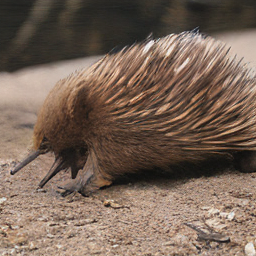
\includegraphics[width=0.145\linewidth]{028102-class0102.png}
    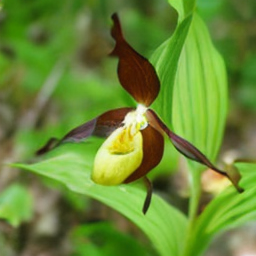
\includegraphics[width=0.145\linewidth]{009986-class0986.png}
    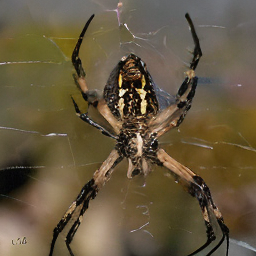
\includegraphics[width=0.145\linewidth]{028072-class0072.png}
    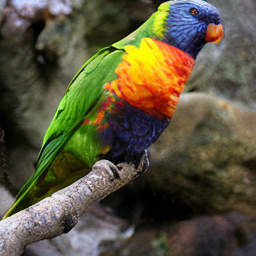
\includegraphics[width=0.145\linewidth]{023090-class0090.png}
    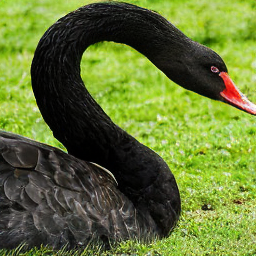
\includegraphics[width=0.145\linewidth]{044100-class0100.png}
    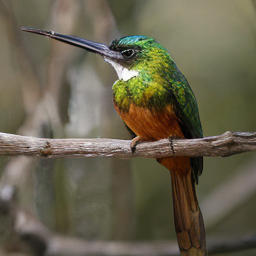
\includegraphics[width=0.145\linewidth]{037095-class0095.png}

    \vspace{0.25em}

    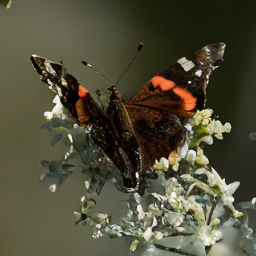
\includegraphics[width=0.145\linewidth]{007321-class0321.png}
    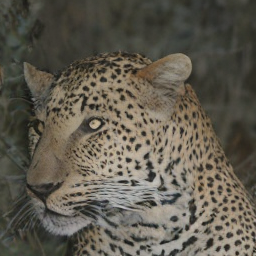
\includegraphics[width=0.145\linewidth]{043288-class0288.png}
    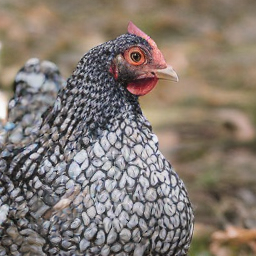
\includegraphics[width=0.145\linewidth]{013008-class0008.png}
    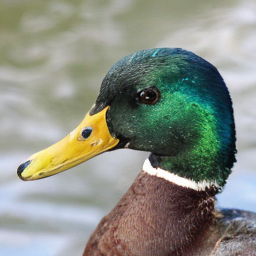
\includegraphics[width=0.145\linewidth]{021097-class0097.png}
    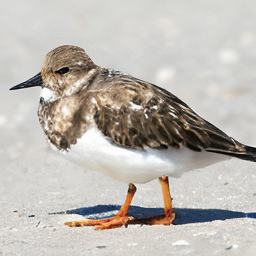
\includegraphics[width=0.145\linewidth]{015139-class0139.png}
    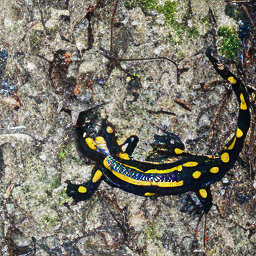
\includegraphics[width=0.145\linewidth]{024025-class0025.png}

    \vspace{0.45em}
    {\scriptsize نمونه‌های تولیدشده توسط \duo{} روی کلاس‌های مختلف \imagenet{}.}
\end{frame}

\begin{frame}{مقایسه کیفی با مدل پایه}
    \begin{columns}[onlytextwidth]
        \begin{column}{0.49\textwidth}
            \centering
            {\bfseries \lr{Base DiT}}\\[0.25em]
            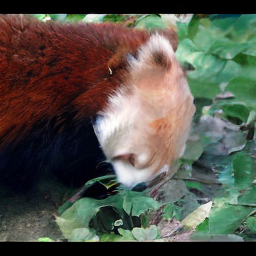
\includegraphics[width=0.23\linewidth]{comparison_samples/dit017387-class0387.png}
            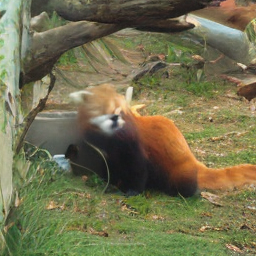
\includegraphics[width=0.23\linewidth]{comparison_samples/dit018387-class0387.png}
            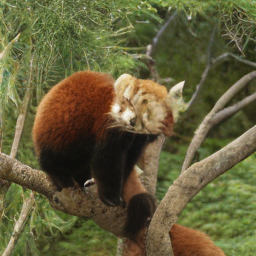
\includegraphics[width=0.23\linewidth]{comparison_samples/dit019387-class0387.png}
            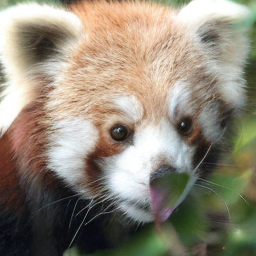
\includegraphics[width=0.23\linewidth]{comparison_samples/dit045387-class0387.png}\\[-0.1em]
            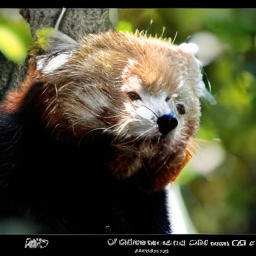
\includegraphics[width=0.23\linewidth]{comparison_samples/dit046387-class0387.png}
            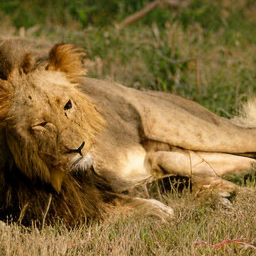
\includegraphics[width=0.23\linewidth]{comparison_samples/dit.png}
            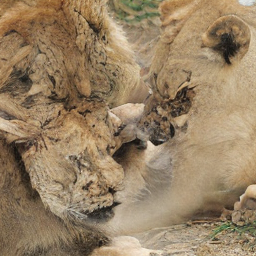
\includegraphics[width=0.23\linewidth]{comparison_samples/dit1.png}
        \end{column}
        \begin{column}{0.49\textwidth}
            \centering
            {\bfseries \duo{}}\\[0.25em]
            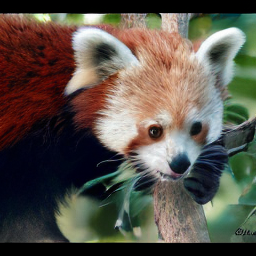
\includegraphics[width=0.23\linewidth]{comparison_samples/duodit017387-class0387.png}
            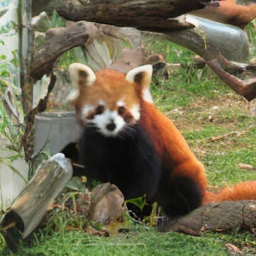
\includegraphics[width=0.23\linewidth]{comparison_samples/duodit018387-class0387.png}
            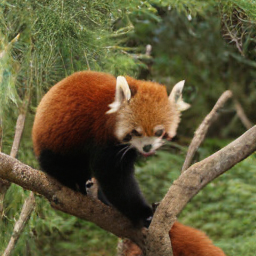
\includegraphics[width=0.23\linewidth]{comparison_samples/duodit019387-class0387.png}
            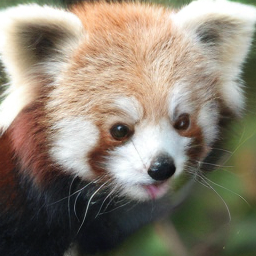
\includegraphics[width=0.23\linewidth]{comparison_samples/duodit045387-class0387.png}\\[-0.1em]
            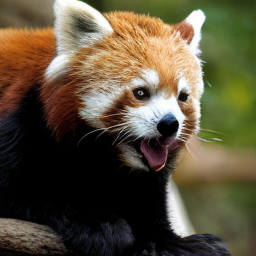
\includegraphics[width=0.23\linewidth]{comparison_samples/duodit046387-class0387.png}
            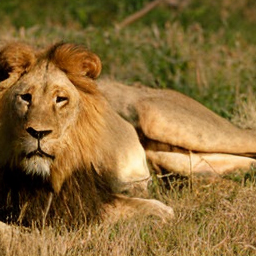
\includegraphics[width=0.23\linewidth]{comparison_samples/doudit.png}
            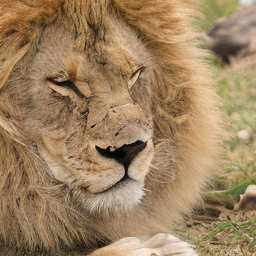
\includegraphics[width=0.23\linewidth]{comparison_samples/doudit1.png}
        \end{column}
    \end{columns}
    \vspace{0.25em}
    {\scriptsize نمونه های مقایسه ایی برای هر مدل}
\end{frame}

\begin{frame}{مطالعه انسانی}
    \begin{columns}[onlytextwidth]
        \begin{column}{0.47\textwidth}
            \begin{itemize}
                \compactitems
                \item ۱۳ شرکت‌کننده
                \item ۳۰۰ مقایسه زوجی برای هر نفر
                \item مجموع ۳۹۰۰ پاسخ
                \item مقایسه بین \duo{} و \lr{LightningDiT}
            \end{itemize}
        \end{column}
        \begin{column}{0.49\textwidth}
            \begin{latin}
            \begin{tabular}{lcc}
                \toprule
                Choice & Count & Percent\\
                \midrule
                DuoDiT & 1593 & 40.85\%\\
                LightningDiT & 1398 & 35.85\%\\
                Tie & 909 & 23.31\%\\
                \midrule
                DuoDiT pref. & \multicolumn{2}{c}{53.26\%}\\
                \bottomrule
            \end{tabular}
            \end{latin}
        \end{column}
    \end{columns}
    % \vspace{0.5em}
    % {\small ترجیح \duo{} روی مقایسه‌های محاسبه شده است.}
\end{frame}

\begin{frame}{هزینه محاسباتی}
    \centering
    \begin{latin}
    \begin{tabular}{lccccc}
        \toprule
        Method & GFLOPs & Params & Trainable & Time/Epoch & VRAM\\
        \midrule
        DuoDiT-200 & 267.10 & 690.39M & 17.95M & 13m & 2.91GB\\
        FineDiffusion & 228.84 & 685.64M & 12.15M & 22m & 3.19GB\\
        \bottomrule
    \end{tabular}
    \end{latin}
    \vspace{0.9em}
    \begin{duobox}{تفسیر}
        \duo{}
        پارامتر آموزش‌پذیر بیشتری از 
        \lr{FineDiffusion}
        دارد اما زمان هر ایپاک و بیشینه حافظه مصرفی کمتری نسبت به آن دارد.
        همچین نتایج کمی و کیفی به وضوح بهتری دارد.
    \end{duobox}
\end{frame}

\begin{frame}{مطالعه حذفی: راهبرد تجمیع}
    \centering
    \begin{latin}
    \begin{tabular}{lccc}
        \toprule
        Strategy & FID \(\downarrow\) & KID \(\downarrow\) & LPIPS-Mean \(\downarrow\)\\
        \midrule
        Average Pooling & 142.31 & 0.0452 & 0.7489\\
        Max Pooling & 140.85 & 0.0438 & 0.7412\\
        Linear Projection & 138.92 & 0.0415 & 0.7352\\
        Local CLS Token & \textbf{135.78} & \textbf{0.0396} & \textbf{0.7018}\\
        \bottomrule
    \end{tabular}
    \end{latin}
    \vspace{0.8em}
    \begin{duobox}{نتیجه}
        توکن کلاس محلی از قواعد ثابت pooling بهتر عمل می‌کند، چون تجمیع را وابسته به محتوای همان ناحیه انجام می‌دهد.
    \end{duobox}
\end{frame}

\begin{frame}{مطالعه حذفی: عمق و \cfg{}}
    \begin{columns}[onlytextwidth]
        \begin{column}{0.49\textwidth}
            \centering
            {\bfseries عمق شاخه دوم}\\[0.3em]
            \begin{latin}
            \begin{tabular}{lccc}
                \toprule
                Variant & GFLOPs & Time & VRAM\\
                \midrule
                1 block & 267.10 & 13m & 2.91GB\\
                2 blocks & 299.32 & 15m & 2.99GB\\
                4 blocks & 363.75 & 26m & 3.15GB\\
                \bottomrule
            \end{tabular}
            \end{latin}
        \end{column}
        \begin{column}{0.49\textwidth}
            \centering
            {\bfseries شاخه دوم و \cfg{}}\\[0.3em]
            \begin{latin}
            \begin{tabular}{lcc}
                \toprule
                Variant & FID & KID\\
                \midrule
                Skip Connection & 216.7914 & 0.0512\\
                ViT features & 215.7946 & 0.0503\\
                \midrule
                CFG=1.0 & 210.3986 & 0.04142\\
                CFG=2.0 & 215.7946 & 0.05030\\
                CFG=4.0 & 230.0816 & 0.06270\\
                \bottomrule
            \end{tabular}
            \end{latin}
        \end{column}
    \end{columns}
\end{frame}

\begin{frame}{بحث و محدودیت‌ها}
    \begin{itemize}
        \compactitems
        \item شاخه ریزدانه به بهبود \kid{} و \lpips{} کمک کرده است.
        \item اگرچه \fid{} نسبت به \lr{LightningDiT} ضعیف‌تر است؛ اما در مطالعات انسانی \lr{DuoDiT} برتری دارد.
        \item شاخه محلی ممکن است در مرزهای مبهم، جزئیات نادرست را نیز تقویت کند.
        \item در برخی از نمونه های خروجی محتوای غیرواقعی دیده می شود.
    \end{itemize}
    \vspace{0.5em}
    \begin{duobox}{تفسیر}
        افزودن مسیر سبک و محلی به \dit{} منجمد میتواند کیفیت ادراکی و کارایی تنظیم دقیق را بهبود دهد.
    \end{duobox}
\end{frame}

\section{پیشنهادات و جمع‌بندی}

\begin{frame}{پیشنهادات پژوهشی}
    \begin{columns}[onlytextwidth]
        \begin{column}{0.48\textwidth}
            \begin{itemize}
                \compactitems
                \item فعال‌سازی \lr{FiLM} برای شرط‌گذاری دقیق‌تر زمان و کلاس.
                \item بررسی دیتاست‌های پیچیده‌تر مانند \lr{iNaturalist}.
            \end{itemize}
        \end{column}
        \begin{column}{0.48\textwidth}
            \begin{itemize}
                \compactitems
                \item کاهش هزینه استنتاج با کوانتیزاسیون یا مسیرهای پویا.
                \item جایگزینی بدنه اصلی یا خبره \vit{} با مدل‌های جدیدتر.
            \end{itemize}
        \end{column}
    \end{columns}
    % \vspace{0.4em}
    % \centering
    % 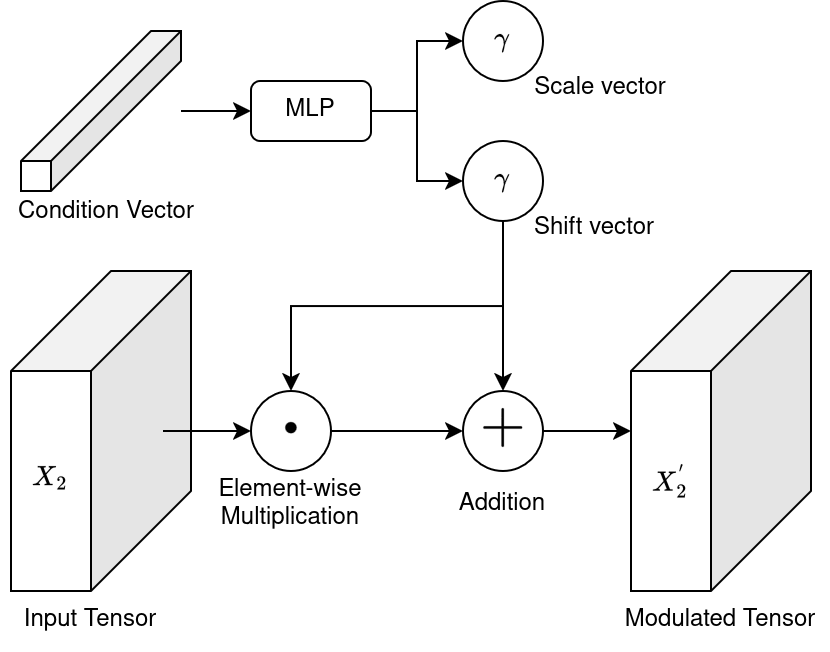
\includegraphics[width=0.48\linewidth,height=0.30\textheight,keepaspectratio]{film_modulation.png}
\end{frame}

\begin{frame}{جمع‌بندی}
    \begin{enumerate}
        \compactitems
        \item \duo{} یک معماری دوجریانی برای تنظیم دقیق پارامتر-کارای \dit{} معرفی می‌کند.
        \item بدنه \lr{DiT-XL/2} منجمد می‌ماند و شاخه \lr{x2} ویژگی‌های محلی را استخراج می‌کند.
        \item توکن کلاس محلی، تجمیع محتوا-آگاه از \(4T\) به \(T\) توکن را انجام می‌دهد.
        \item \duo{} با \lr{17.95M} پارامتر آموزش‌پذیر به \lr{FID=2.219}، \lr{KID=0.0014} و \lr{LPIPS=0.7162} رسیده است.
        \item در مطالعه انسانی، \duo{} در \lr{53.26\%} مقایسه‌های غیرمساوی بر \lr{LightningDiT} ترجیح داده شده است.
    \end{enumerate}
\end{frame}

\begin{frame}{}
    \centering
    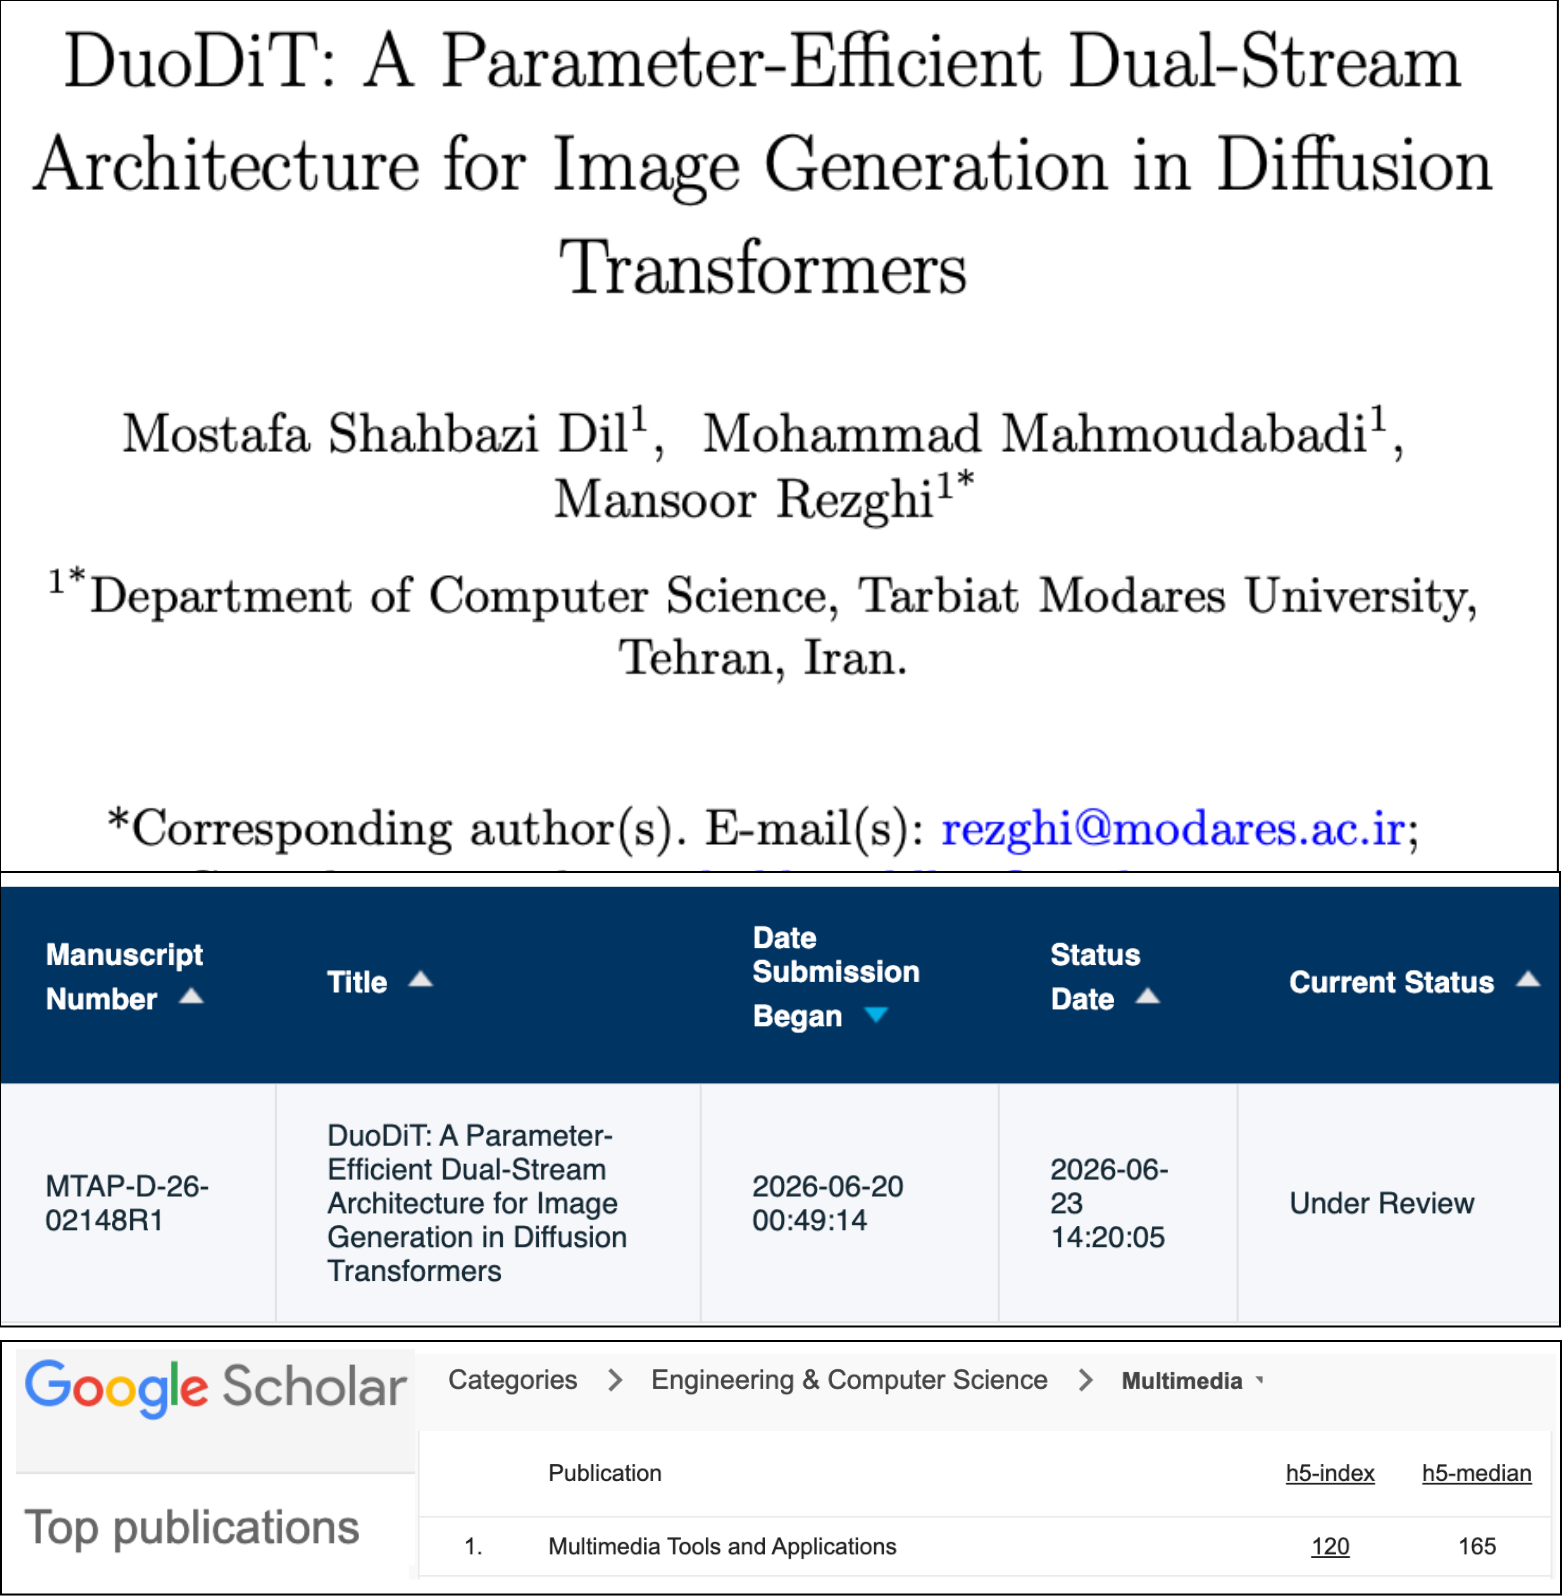
\includegraphics[width=0.95\linewidth,height=0.95\textheight,keepaspectratio]{paper-status.drawio.png}
    \vspace{0.2em}
    \par\medskip
\end{frame}

\begin{frame}[plain]
    \Closure[background=true,circles=true]{سپاسگزارم}{پرسش‌ها؟}
\end{frame}

\DuoAppendixtrue
\appendix

\begin{frame}{تنظیمات آموزش}
    \centering
    \begin{latin}
    \begin{tabular}{llc}
        \toprule
        Category & Parameter & Value\\
        \midrule
        Model & Architecture & DiT-XL/2\\
        Model & Main patch / x2 patch & 2 / 1\\
        Training & Resolution & \(256\times256\)\\
        Training & VAE & sd-vae-ft-ema\\
        Training & Diffusion steps & 1000\\
        Training & Optimizer & AdamW\\
        Training & LR & \(1\times10^{-4}\)\\
        Sampling & DDPM steps & 250\\
        Sampling & CFG scale & 1.5\\
        \bottomrule
    \end{tabular}
    \end{latin}
\end{frame}

\begin{frame}{منابع اصلی}
    \begin{itemize}
        \compactitems
        \item \lr{Kingma \& Welling, 2013}: \lr{VAE}
        \item \lr{Goodfellow et al., 2014}: \lr{GAN}
        \item \lr{Ho et al., 2020}: \lr{DDPM}
        \item \lr{Dosovitskiy et al., 2020}: \lr{Vision Transformer}
        \item \lr{Peebles \& Xie, 2022}: \lr{DiT}
        \item \lr{Bao et al., 2022}: \lr{U-ViT}
        \item \lr{Chen et al., 2021}: \lr{CrossViT}
        \item \lr{He et al., 2016}: \lr{ResNet}
        \item \lr{Dual Diffusion}: \lr{D-DiT}
        \item \lr{DUPA}: \lr{Dual-Path Condition Alignment}
        \item \lr{Unified Local/Global Attention}: \lr{ViT}
        \item \lr{Yao et al., 2025}: \lr{LightningDiT}
        \item \lr{Pan et al., 2024}: \lr{FineDiffusion}
    \end{itemize}
\end{frame}

\end{document}
